\section{Line and Surface Integrals}

	We will introduce two objects: \textit{vector fields} as the thing that we are trying to integrate, and \textit{parameterized sets} as the thing we are integrating over. 
	
\subsection{Vector Fields}

  \begin{definition}[Gradient]
		The \textbf{gradient} of differentiable $f: E \subset \mathbb{R}^n \to \mathbb{R}$ is the vector field defined in the equivalent ways: 
		\begin{enumerate}
		  \item \textit{Vector of Partials}. The gradient is
				\begin{equation}
					\nabla f: E \to \mathbb{R}^n, \qquad \nabla f(x) \coloneqq \begin{pmatrix} \frac{\partial f}{\partial x_1} (x) \\ \vdots \\ \frac{\partial f}{\partial x_n} (x) \end{pmatrix}
				\end{equation}

			\item \textit{Coordinate-Free}. It is the unique vector field whose dot product with any vector $v$ at each point is the directional derivative of $f$ along $v$. That is, 
				\begin{equation}
					\nabla f_a \cdot v = D f_a v \text{ for all } a \in D
				\end{equation}
		\end{enumerate}
  \end{definition}
	\begin{proof}
	  
	\end{proof}

  Note that the gradient is a vector field (a bundle of vectors), while the total derivative is a covector field (a bundle of covectors). Since $\mathbb{R}^n$ is an inner product space, we can invoke Riesz Representation theorem and see that they are related in the way that 
	\begin{equation}
  	D f_a v = \nabla f (a) \cdot v
	\end{equation}
  where $\cdot$ represents the dot product. At this point, it's a bit hard to see the difference between these two, but in more abstract spaces the total derivative generalizes much better than the gradient, which exists for inner product spaces. From this, we can write a coordinate independent definition of the gradient. 

  \begin{lemma}[Gradient as Direction of Fastest Increase]
		Let $f$ be a real-valued function such that $\nabla f(x) \neq 0$. Then, at the point $x$, 
		\begin{enumerate}
		  \item $\nabla f(x)$ points in the direction along which $f$ is increasing the fastest. 
			\item $-\nabla f(x)$ points in the direction along which $f$ is decreasing the fastest. 
		\end{enumerate}
  \end{lemma}
  \begin{proof}
		Note that this is a coordinate-independent proof. Given a directional vector $v$, we can normalize it since we are only interested in direction. Evaluating it with the total derivative at $x$ gives us $D_a f v$. But by definition, 
		\begin{equation}
			\nabla f_a \cdot v = D f_a v
		\end{equation}
		which means that 
		\begin{align}
			\sup_{\|v\| = 1} \{D f_a v\} 
				& = \sup_{\|v\|=1} \{\nabla f_a \cdot v\} \\
				&  = \sup_{\|v\|=1} \{ \|\nabla f_a\| \, \|v\| \cos(\theta)\} \\
				& = \sup \{\|\nabla f_a\| \cos(\theta)\} \\
				& = \|\nabla f_a\| \text{ when } \theta = 0
		\end{align}
		Therefore, $v$ must point in the direction of $\nabla f_a$. 
  \end{proof}

  Therefore, we can interpret the gradient evaluated at a point as the tangent vector that points in the direction of fastest increase. We can also interpret the gradient $\nabla f$ itself as the vector field that determines some sort of "flow" in the domain $\mathbb{R}^n$. Therefore, if we drop a point in this field, the point will flow through $\mathbb{R}^n$ through a current determined by $\nabla f$ and will eventually end up at a local maximum. 

  \begin{definition}[Del Operator]
		The \textbf{del operator} is notational shorthand used to represent the following operations. 
		\begin{enumerate}
			\item \textit{Gradient}. Given $f: \mathbb{R}^n \to \mathbb{R}$, $\nabla f$ represents the gradient. 

			\item \textit{Dot Product}. 
				Given $F: \mathbb{R}^n \to \mathbb{R}^n$, by abuse of notation from treating $\nabla$ as a vector, we can define 
				\begin{equation}
					\nabla \cdot F \coloneqq \begin{pmatrix} \frac{\partial}{\partial x_1} \\ \vdots \\ \frac{\partial}{\partial x_n} \end{pmatrix} \cdot \begin{pmatrix} F_1 \\ \vdots \\ F_n \end{pmatrix} = \sum_i \frac{\partial F_i}{\partial x_i}
				\end{equation}

				\item \textit{Cross Product}. Given $F: \mathbb{R}^3 \to \mathbb{R}^3$, by abuse of notation from treating $\nabla$ as a vector, we can define 
				\begin{equation}
					\nabla \times F \coloneqq \begin{pmatrix} \frac{\partial}{\partial x_1} \\ \frac{\partial}{\partial x_2} \\ \frac{\partial}{\partial x_3} \end{pmatrix} \cdot \begin{pmatrix} F_1 \\ F_2 \\ F_3 \end{pmatrix} = 
				\end{equation}
		\end{enumerate}

		For convenience, we use the del operator to denote the gradient. The \textbf{del operator} $\nabla: f \mapsto \nabla f$ takes in a differentiable function and outputs the gradient of it. 
  \end{definition}

  We would like to observe some nice properties of vector fields. Two natural properties can be analyzed through the divergence and curl. Colloquially, the divergence is an operator $\Div$ that operates on a vector field and produces a scalar field which provides the quantity of the vector field's source at each point. Technically, the divergence represents the volume density of the outward flux of a vector field from an infinitesimal volume around a given point. 

  \begin{definition}[Divergence]
		The \textbf{divergence} of a vector field $F: \mathbb{R}^n \to \mathbb{R}^n$ is a scalar field defined 
		\begin{equation}
		  \Div F \coloneqq \nabla \cdot F
		\end{equation}

		\begin{figure}[H]
			\centering
			\pgfplotsset{width=6.5cm, compat=1.16}
			% SUBFIGURE A: Positive Divergence (Source)
			\begin{subfigure}[b]{0.32\textwidth}
				\centering
				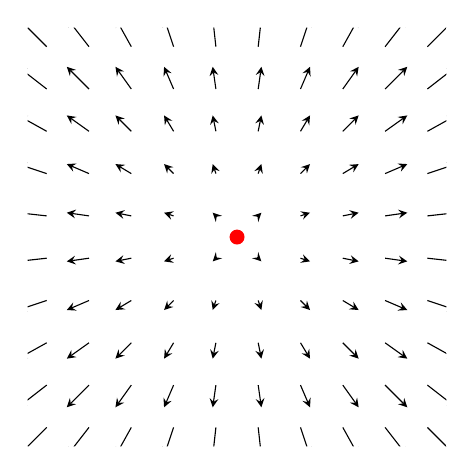
\begin{tikzpicture}
					\begin{axis}[
						view={0}{90},
						domain=-2:2,
						domain y=-2:2,
						hide axis,
						xmin=-2.2, xmax=2.2,
						ymin=-2.2, ymax=2.2,
						zmin=-1, zmax=1,
						axis equal image
					]
						\addplot3[
							black,
							-stealth,
							samples=10,
							quiver={
								u={x},
								v={y},
								scale arrows=0.15,
							},
						] {0};
						% Red point marked at the origin
						\addplot3[only marks, mark=*, mark size=2.5pt, color=red] coordinates {(0,0,0)};
					\end{axis}
				\end{tikzpicture}
				\caption{$\nabla \cdot F > 0$ (Source)}
				\label{fig:positive_div}
			\end{subfigure}
			\hfill 
			% SUBFIGURE B: Negative Divergence (Sink)
			\begin{subfigure}[b]{0.32\textwidth}
				\centering
				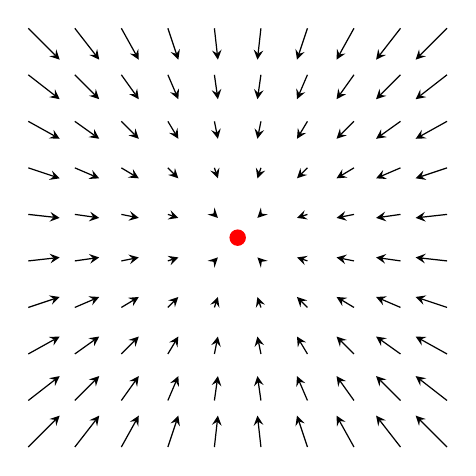
\begin{tikzpicture}[scale=1.1]
					\begin{axis}[
						view={0}{90},
						domain=-2:2,
						domain y=-2:2,
						hide axis,
						xmin=-2.2, xmax=2.2,
						ymin=-2.2, ymax=2.2,
						zmin=-1, zmax=1,
						axis equal image
					]
						\addplot3[
							black,
							-stealth,
							samples=10,
							quiver={
								u={-x},
								v={-y},
								scale arrows=0.15,
							},
						] {0};
						% Red point marked at the origin
						\addplot3[only marks, mark=*, mark size=2.5pt, color=red] coordinates {(0,0,0)};
					\end{axis}
				\end{tikzpicture}
				\caption{$\nabla \cdot F < 0$ (Sink)}
				\label{fig:negative_div}
			\end{subfigure}
			\hfill 
			% SUBFIGURE C: Zero Divergence (Uniform Field)
			\begin{subfigure}[b]{0.32\textwidth}
				\centering
				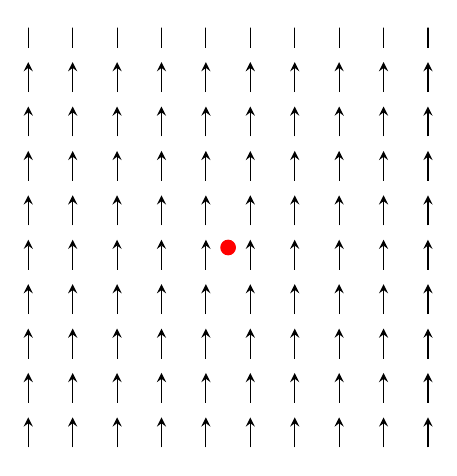
\begin{tikzpicture}[scale=1.05]
					\begin{axis}[
						view={0}{90},
						domain=-2:2,
						domain y=-2:2,
						hide axis,
						xmin=-2.2, xmax=2.2,
						ymin=-2.2, ymax=2.2,
						zmin=-1, zmax=1,
						axis equal image
					]
						\addplot3[
							black,
							-stealth,
							samples=10,
							quiver={
								u={0},
								v={1},
								scale arrows=0.3,
							},
						] {0};
						% Red point marked at the origin
						\addplot3[only marks, mark=*, mark size=2.5pt, color=red] coordinates {(0,0,0)};
					\end{axis}
				\end{tikzpicture}
				\caption{$\nabla \cdot F = 0$ (Constant)}
				\label{fig:zero_div}
			\end{subfigure}
			\caption{ Imagine that the vector field $F$ represents fluid flow in $\mathbb{R}^n$. Divergence is then the measure of the net amount of fluid flowing in and out of an infinitesimally small region, labeled at each point. If the net fluid flow is positive (i.e. more fluid is flowing in than out) at point $x_0$, then $\Div{F}(x_0) > 0$. If the net fluid flow is negative (i.e. more fluid is flowing out than in) at point $x_0$, then $\Div{F}(x_0) < 0$. Therefore, each point either acts as a "source" of fluid emanating from it or as a "sink" that sucks in more fluid than it puts out. }
			\label{fig:divergence_comparison}
		\end{figure}
  \end{definition}

	When $n = 1$, $F$ reduces to a regular function and $\Div F$ reduces to the ordinary derivative. 

	\begin{lemma}[Linearity of Divergence]
		By linearity of partials, $\Div$ is also a linear operator. That is, given two vector fields $F, G$ and two scalars $\alpha, \beta$, 
		\begin{equation}
			\Div (\alpha F + \beta G) = \alpha \Div F + \beta \Div G
		\end{equation}
	\end{lemma}
	\begin{proof}
	  
	\end{proof}

	\begin{lemma}[Product Rule]
		Divergence satisfies the product rule: Given a vector field $F: \mathbb{R}^n \to \mathbb{R}^n$ and a scalar function $\varphi: \mathbb{R}^n \to \mathbb{R}$. 
		\begin{equation}
			\nabla \cdot (\varphi F) = \nabla \varphi \cdot F + \varphi (\nabla \cdot F)
		\end{equation}
	\end{lemma}
	\begin{proof}
	  
	\end{proof}

  \begin{lemma}[Divergence in Cylindrical Coordinates]
		For vector field $F: \mathbb{R}^3 \to \mathbb{R}^3$ expressed in cylindrical coordinates as 
		\begin{equation}
			F = \begin{pmatrix} F_r \\ F_\theta \\ F_z \end{pmatrix}
		\end{equation}
		the divergence is
		\begin{equation}
			\Div F = \nabla \cdot F = \frac{1}{r} \frac{\partial}{\partial r} \big(r F_r \big) + \frac{1}{r} \frac{\partial F_\theta}{\partial \theta} + \frac{\partial F_z}{\partial z}
		\end{equation}
		Note that the condition of locality is important, since in general a global cylindrical coordinate system would be inconsistent. 
  \end{lemma}
	\begin{proof}
	  
	\end{proof}

  \begin{lemma}[Divergence in Spherical Coordinates]
		For vector field $F: \mathbb{R}^3 \to \mathbb{R}^3$ expressed in spherical coordinates $(r, \theta, \phi)$, the divergence is 
		\begin{equation}
			\Div F = \nabla \cdot F = \frac{1}{r^2} \frac{\partial}{\partial r} \big( r^2 F_r) + \frac{1}{r \, \sin{\theta}} \frac{\partial}{\partial \theta} \big( \sin{\theta} F_\theta\big) + \frac{1}{r\, \sin{\theta}} \frac{\partial F_\phi}{\partial \phi}
		\end{equation}
  \end{lemma}
	\begin{proof}
	  
	\end{proof}

  \begin{example}[Solenoidal Vector Fields]
		A vector field $F: \mathbb{R}^n \to \mathbb{R}^n$ is \textbf{solenoidal}, or \textbf{incompressible}, if $\Div F = 0$ for all $x \in \mathbb{R}^n$.\footnote{So, $F$ has no sources or sinks.}

		\begin{figure}[H]
			\centering 
			\pgfplotsset{width=8cm,compat=1.16}
			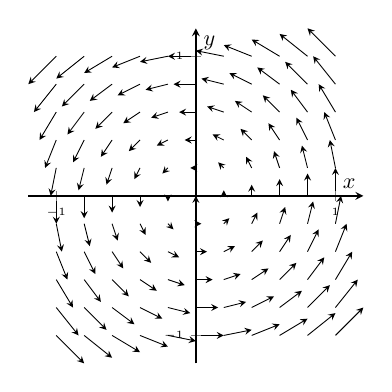
\begin{tikzpicture}[scale=0.8]
				\begin{axis}[
					view={0}{90},
					domain=-1:1,
					domain y=-1:1,
					axis lines=middle,
					xmin=-1.2, xmax=1.2,
					ymin=-1.2, ymax=1.2,
					zmin=-1, zmax=1,
					xtick={-2.0, -1.0, 0.0, 1.0, 2.0},
					ytick={-2.0, -1.0, 0.0, 1.0, 2.0},
					xticklabel style={/pgf/number format/fixed, /pgf/number format/precision=1},
					yticklabel style={/pgf/number format/fixed, /pgf/number format/precision=1},
					xlabel={$x$},
					ylabel={$y$},
					axis equal image,
					inner axis line style={black, semithick},
					tick label style={font=\tiny}
				]
					\addplot3[
						black,
						-stealth,
						samples=11,
						quiver={
							u={-y},
							v={x},
							scale arrows=0.2,
						},
					] {0};
				\end{axis}
			\end{tikzpicture}
			\caption{The vector field $F: (x, y) \mapsto (y, -x)$ is solenoidal. } 
			\label{fig:solenoidal_vector_field}
		\end{figure}
  \end{example}

  Colloquially, the curl is a vector operator that describes the infinitesimal circulation of a vector field in $3$-dimensional Euclidean space, where the curl at each point is represented by a vector whose length and direction denote the magnitude and axis as the maximum circulation. That is, if one drops a twig or a ball with its center of mass at a certain point, the curl measures how much it will spin. In physics, the rotation of a rigid body in 3-dimensions can be described by a vector $\omega$ along the axis of rotation. $\omega$ is called the \textit{angular velocity vector}, with $\|\omega\|$ denoting the angular speed of the body. The curl of this vector field measured at the center of mass of the body is measured as $2 \omega$. That is, the curl outputs \textit{twice} the angular velocity vector of any rigid body. Note that unlike the gradient and divergence operators, curl does not generalize as simply to other dimensions. 

  \begin{definition}[Curl]
		The \textbf{curl} of a differentiable vector field $F: \mathbb{R}^3 \to \mathbb{R}^3$ is an operator
		\begin{equation}
			\curl{F} \coloneqq \nabla \times F
		\end{equation}
  \end{definition}

  \begin{example}[Irrotational Vector Fields]
		A vector field $F$ is \textbf{irrotational} if $\curl{F} = 0$.\footnote{Visually, this indicates that there are no "whirlpools" everywhere, meaning that any rigid body placed anywhere, while it may travel along a path, will not rotate around its own axis. } 
  \end{example}

  It has been shown that fluid draining from a tub is usually irrotational except for right at the center, which is surprising since the fluid itself is "rotating" around the drain. 

	\begin{theorem}[Curl Fields Have no Divergence]
		For any $C^2$ vector field $F: \mathbb{R}^3 \to \mathbb{R}^3$, 
		\begin{equation}
			\Div{\curl{F}} = \nabla\cdot (\nabla \times F) = 0
		\end{equation}
		That is, the divergence of any curl is 0. 
  \end{theorem}
  \begin{proof}
		Proved by equality of mixed partials. 
  \end{proof}

	\begin{definition}[Laplacian]
		The \textbf{Laplacian} of a function $f: \mathbb{R}^n \to \mathbb{R}$ is the divergence of the gradient. 
		\begin{equation}
			\nabla^2 f \coloneqq \nabla \cdot (\nabla f) = \sum_{i=1}^n \frac{\partial^2 f}{\partial x_i^2}
		\end{equation}
  \end{definition}

  \begin{definition}[Conservative Vector Fields]
		A vector field $F: U \subset \mathbb{R}^n \to \mathbb{R}^n$ is a \textbf{conservative vector field} if and only if there exists a scalar field $f: U \subset \mathbb{R}^n \to \mathbb{R}$ such that 
		\begin{equation}
			F = \nabla f
		\end{equation}
		on $U$. 

		\begin{figure}[H]
			\centering
			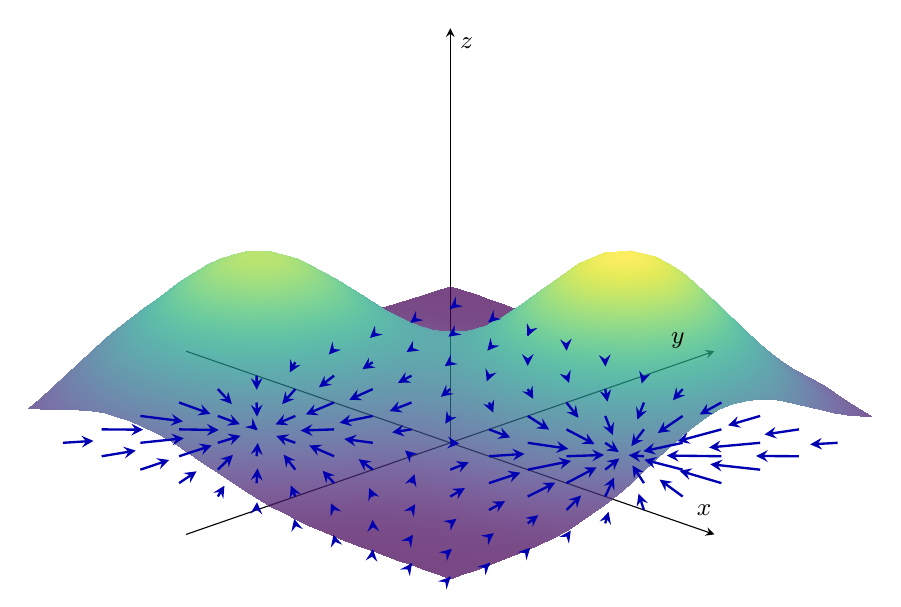
\begin{tikzpicture}[scale=1.0]
				\begin{axis}[
					view={45}{32},
					axis lines=center,
					xlabel={$x$},
					ylabel={$y$},
					zlabel={$z$},
					xmin=-3, xmax=3,
					ymin=-3, ymax=3,
					zmin=0, zmax=4.8,
					domain=-2.4:2.4,
					y domain=-2.4:2.4,
					samples=34,
					samples y=34,
					width=15cm,
					height=11.5cm,
					grid=major,
					ticks=none,
					tick label style={font=\small},
					label style={font=\small},
					colormap/viridis,
					clip=false
				]
					\addplot3[
						surf,
						opacity=0.72,
						shader=interp,
						draw=black!20
					]
					{2.2*exp(-((x-1.2)^2 + (y-0.8)^2)/1.6)
					+ 1.9*exp(-((x+1.3)^2 + (y+0.9)^2)/1.8)
					+ 0.12};

					\addplot3[
						blue!70!black,
						-stealth,
						samples=11,
						samples y=11,
						domain=-2.2:2.2,
						y domain=-2.2:2.2,
						quiver={
							u={-2.75*(x-1.2)*exp(-((x-1.2)^2 + (y-0.8)^2)/1.6)
								-2.11*(x+1.3)*exp(-((x+1.3)^2 + (y+0.9)^2)/1.8)},
							v={-2.75*(y-0.8)*exp(-((x-1.2)^2 + (y-0.8)^2)/1.6)
								-2.11*(y+0.9)*exp(-((x+1.3)^2 + (y+0.9)^2)/1.8)},
							w={0},
							scale arrows=0.3,
							every arrow/.append style={line width=0.85pt}
						}
					]
					(x,y,0);
				\end{axis}
			\end{tikzpicture}
			\caption{If vector field $F$ is conservative, then there exists a smooth scalar function $f$ such that $\nabla f = F$. For each latitude and longitude on a certain map, we can give it an altitude as a function of those coordinates (picture a map with a bunch of hills and valleys). The gradient and thus the vector field is all the vectors that point in the direction of highest ascent. The vector field is all the vectors that point in the direction of highest ascent. }
			\label{fig:conservative_gradient_surface}
		\end{figure}
  \end{definition}

  Conservative vector fields appear naturally in mechanics: they are vector fields representing forces of physical systems in which energy is conserved. 

	\begin{theorem}[Gradient Fields Have No Curl]
		Given a $C^2$-function $f: \mathbb{R}^3 \to \mathbb{R}$,
		\begin{equation}
			\nabla \times ( \nabla f) = 0
		\end{equation}
		That is, the curl of any gradient vector field is the zero vector. 
  \end{theorem}
  \begin{proof}
		$\nabla \times \nabla f$ can be expanded to
		\begin{equation} 
			\begin{pmatrix}
				\frac{\partial^2 f}{\partial y \partial z} - \frac{\partial^2 f}{\partial z \partial y} \\ 
				\frac{\partial^2 f}{\partial z \partial x} - \frac{\partial^2 f}{\partial x \partial z} \\
				\frac{\partial^2 f}{\partial x \partial y} - \frac{\partial^2 f}{\partial y \partial x}
			\end{pmatrix} = \begin{pmatrix}
			  0 \\ 0 \\ 0
			\end{pmatrix}
		\end{equation}
		by equality of mixed partials. 
  \end{proof}

  \begin{theorem}[Helmholtz Decomposition]
		Let $F: \mathbb{R}^3 \to \mathbb{R}^3$ be a $C^2$ vector field. Then, $F$ can be decomposed into a curl-free component and a divergence-free component. That is, there exists vector fields $A$ and $\Phi$
		\begin{equation}
			F = - \nabla \cdot \Phi + \nabla \times A
		\end{equation}
  \end{theorem}
		
\subsection{Parameterizations and Orientation}

	\begin{definition}[Parameterization]
		Given some subset $E \subset \mathbb{R}^n$, a \textbf{k-parameterization} of $E$ is a continuous surjective map 
		\begin{equation}
		  \varphi: D \subset \mathbb{R}^k \to E
		\end{equation}
		where $D$ is a compact subset of $\mathbb{R}^k$. 
	\end{definition} 
	
	\begin{definition}[Reparameterization]
		Let $E \subset \mathbb{R}^n$ with parameterization $\varphi: D \subset \mathbb{R}^k \to E$. Given \textbf{reparameterization} of $E$ is a continuous bijective map $h: D^\prime \subset \mathbb{R}^k \to D$, where $D^\prime$ is a compact subset of $\mathbb{R}^k$. Therefore, 
		\begin{equation}
		  \varphi \circ h : D^\prime \to E
		\end{equation} 
		is another parameterization of $E$. 
	\end{definition}
	
	
	Continuity alone is not enough to guarantee that a parameterized set behaves like a curve in the usual geometric sense. In fact, we will sketch a construction of a continuous surjective map $\gamma : [0,1] \to [0,1]^2$, called a \textit{space-filling curve}. 
	
	\begin{example}[Space-Filling Curve in $\mathbb{R}^2$]
		Let $C \subset [0,1]$ be the Cantor set. Every point $x \in C$ has a ternary expansion using only the digits $0$ and $2$. 
		\begin{equation}
			x = 0.a_1a_2a_3\cdots, \qquad a_i \in \{0,2\}.
		\end{equation}
		Define binary digits $b_i = \frac{a_i}{2} \in \{0,1\}$. Now split the binary digits into odd and even positions, and define
		\begin{equation}
			\Gamma(x) = \big(
				0.b_1b_3b_5\cdots_2,
				0.b_2b_4b_6\cdots_2
			\big) =
			\bigg(
				\sum_{j=1}^{\infty} \frac{b_{2j-1}}{2^j},
				\sum_{j=1}^{\infty} \frac{b_{2j}}{2^j}
			\bigg).
		\end{equation}
		We claim that $\Gamma: C \to [0, 1]^2$ is continuous and surjective. 
		\begin{enumerate}
		  \item \textit{Continuous}. The idea is that if two Cantor points $x, x^\prime$ are close, then their tenary expansions will agree for a long time. Fix $\epsilon > 0$. Choose $N$ large enough so that
				\begin{equation}
					\sum_{j > N/2} \frac{1}{2^j} < \epsilon.
				\end{equation}
				If two points $x,x'^\prime \in C$ agree in their first $N$ ternary digits, then the corresponding binary digits $b_i,b_i'$ also agree for $1 \leq i \leq N$. Hence the first $\lfloor N/2 \rfloor$ binary digits of both coordinates of $\Gamma(x)$ and $\Gamma(x')$ agree. Therefore
				\begin{equation}
					\|\Gamma(x)-\Gamma(x^\prime)\|_\infty \leq \sum_{j > N/2} \frac{1}{2^j} < \epsilon.
				\end{equation}
				Since agreement of sufficiently many initial ternary digits is guaranteed whenever $x,x^\prime \in C$ are sufficiently close, $\Gamma$ is continuous.
			
			\item \textit{Surjective}. Take any point $(y,z) \in [0,1]^2$, Write $y$ and $z$ in binary:
				\begin{equation}
					y = 0.c_1c_2c_3\cdots_2,
					\qquad
					z = 0.d_1d_2d_3\cdots_2,
				\end{equation}
				where $c_i,d_i \in \{0,1\}$. Now interleave these digits to define
				\begin{equation}
					b_1 = c_1,\quad b_2 = d_1,\quad b_3 = c_2,\quad b_4 = d_2,
					\quad \ldots
				\end{equation}
				Then define
				\begin{equation}
					x = 0.(2b_1)(2b_2)(2b_3)(2b_4)\cdots_3.
				\end{equation}
				Since the ternary digits of $x$ are only $0$ and $2$, we have $x \in C$.
				By construction,
				\begin{equation}
					\Gamma(x) = (y,z).
				\end{equation}
		\end{enumerate}
		
		Finally, we extend $\Gamma$ from $C$ to all of $[0,1]$. 
		\begin{enumerate}
		  \item On $C$, define
				\begin{equation}
					\gamma(t) = \Gamma(t), \qquad t \in C.
				\end{equation}
			
			\item On $[0, 1] \setminus C$, note that this complement is a union of disjoint open intervals. On each such gap $(a,b)$, define $\gamma$ by linearly interpolating between the endpoint values $\Gamma(a)$ and $\Gamma(b)$:
				\begin{equation}
					\gamma(t) = \frac{b-t}{b-a}\Gamma(a) + \frac{t-a}{b-a}\Gamma(b), \qquad t \in (a,b).
				\end{equation}
				Since $[0, 1]^2$ is a convex set, $\gamma$ will land in $[0, 1]^2$. 
		\end{enumerate}
			
		It remains to check that the extension is continuous. On each gap $(a,b)$, the map $\gamma$ is affine in $t$, hence continuous. Moreover, as $t \to a^+$,
		\begin{equation}
			\gamma(t) = \frac{b-t}{b-a}\Gamma(a) + \frac{t-a}{b-a}\Gamma(b) \to \Gamma(a) = \gamma(a),
		\end{equation}
		and similarly $\gamma(t)\to \Gamma(b)=\gamma(b)$ as $t\to b^-$.
			
		Finally, let $c\in C$. Since $C$ is compact and $\Gamma$ is continuous, $\Gamma$ is uniformly continuous on $C$. Hence, given $\epsilon>0$, there exists $\delta>0$ such that whenever $p,q\in C$ and $|p-q|<\delta$, we have
		\begin{equation}
			\|\Gamma(p)-\Gamma(q)\|<\epsilon.
		\end{equation}
		If $t$ is sufficiently close to $c$, then either $t\in C$, in which case $\gamma(t)=\Gamma(t)$ is close to $\Gamma(c)$, or $t$ lies in a gap $(a,b)$ whose endpoints $a,b\in C$ are close to $c$. In the latter case, $\gamma(t)$ is a convex combination of $\Gamma(a)$ and $\Gamma(b)$, both of which are close to $\Gamma(c)$. Therefore $\gamma(t)$ is close to $\Gamma(c)=\gamma(c)$. Thus $\gamma$ is continuous on all of $[0,1]$.
	\end{example}
			
	This shows that a continuous $1$-parameterization can have a $2$-dimensional image. Thus continuity alone is not enough for a useful geometric theory of curves and surfaces. We must make sure that the set $E$ is smooth in the sense that (informally) there aren't any wrinkles, points, folds, or self-intersections in such a way that the tangent plane to the surface is not well-defined. 
			
	\begin{definition}[Regular Parameterization]
		Let $E \subset \mathbb{R}^n$. A \textbf{regular $k$-parameterization} of $E$ is a continuously differentiable surjective map
		\begin{equation}
			\varphi : D \subset \mathbb{R}^k \to E,
		\end{equation}
		where $D$ is compact and where $D\varphi_p : \mathbb{R}^k \to \mathbb{R}^n$ has rank $k$ for every interior point $u \in D$.
	\end{definition}
			
	Note that a parameterization is not necessarily a homeomorphism. It may fail to be injective, and its image may have self-intersections or other singular behavior. If $\varphi$ is a continuous bijection from compact $D$ onto $E \subset \mathbb{R}^n$, then $\varphi$ is a homeomorphism onto $E$. In general, however, a parameterized set should not automatically be regarded as a manifold.
			
	There are many special cases of surfaces, most notably $1$-dimensional paths in $\mathbb{R}^2$ and $\mathbb{R}^3$, along with $2$-dimensional surfaces in $\mathbb{R}^3$. 
			
	\begin{definition}[Curve]
	  A \textbf{parameterized curve} is a $C^1$ surjective map 
		\begin{equation}
			\varphi: [a, b] \subset \mathbb{R} \to E \subset \mathbb{R}^n
		\end{equation} 
		A \textbf{curve} is the image $\varphi([a, b]) \subset \mathbb{R}^n$. 
			
		\begin{enumerate}
			\item $\varphi$ is \textbf{closed} if $\varphi(a) = \varphi(b)$. 
			\item $\varphi$ is \textbf{simple} if the restriction of $\varphi$ to $[a, b)$ is injective.\footnote{Visually, the curve doesn't intersect itself except possible at the endpoints.}
		\end{enumerate}
	\end{definition}
			
	\begin{definition}[Surface]
	  A \textbf{parameterized surface} is a $C^1$ surjective map 
		\begin{equation}
			\varphi: [a_1, b_1] \times [a_2, b_2] \subset \mathbb{R}^2 \to E \subset \mathbb{R}^n
		\end{equation}
		A \textbf{surface} is the image $E$. 
	\end{definition}
	In lower dimensions, we can find some motivation for the tangent space of a paramaterized set. 
			
	\begin{figure}[H]
		\centering 
		\begin{tikzpicture}[scale=0.9, >=Latex, line cap=round, line join=round]
			% Left uv-axes
			\draw[line width=1.2pt, ->] (-5.9,-1.9) -- (-5.9,2.9) node[above] {$v$};
			\draw[line width=1.2pt, ->] (-6.3,-1.2) -- (-2.3,-1.2) node[right] {$u$};
			
			% Domain D
			\draw[line width=1.0pt]
				(-5.05,-0.05)
					.. controls (-5.35,0.35) and (-5.28,0.95) ..
				(-4.95,1.35)
					.. controls (-4.65,1.75) and (-4.2,1.9) ..
				(-3.95,2.15)
					.. controls (-3.78,2.38) and (-3.63,2.65) ..
				(-3.18,2.68)
					.. controls (-2.7,2.7) and (-2.48,2.45) ..
				(-2.35,2.1)
					.. controls (-2.15,1.6) and (-2.08,1.0) ..
				(-2.38,0.58)
					.. controls (-2.62,0.25) and (-2.82,0.18) ..
				(-2.92,-0.28)
					.. controls (-3.08,-0.62) and (-3.45,-0.82) ..
				(-3.78,-0.78)
					.. controls (-4.18,-0.78) and (-4.5,-0.82) ..
				(-4.88,-0.5)
					.. controls (-5.05,-0.35) and (-5.12,-0.22) ..
				cycle;
			
			\coordinate (L) at (-3.45,0.6);
			\fill (L) circle (2.1pt); 
			\node at (-3.15, 0.3) {$x$};
			\draw[blue!85, dotted, line width=0.9pt, ->] (-5.85,0.6) -- (-2.45,0.6);
			\draw[red!80, dotted, line width=0.9pt, ->] (-3.45,-0.9) -- (-3.45,3.15);
			
			% Middle mapping arrows
			\draw[line width=1.0pt, ->] (-1.8,1.35)
				.. controls (-0.6,2.05) and (1.05,2.1) ..
			(2.05,1.72);
			\node at (0.15,2.4) {$\varphi$};
			\draw[red!80, line width=0.9pt, ->] (-1.95,0.15)
				.. controls (-0.45,0.45) and (1.0,0.38) ..
			(2.35,0.25);
			\node[red!80] at (0.18,1.0) {$\dfrac{\partial \varphi}{\partial u}$};
			\draw[blue!85, line width=0.9pt, ->] (-1.95,-0.48)
				.. controls (-0.25,-0.9) and (1.05,-0.98) ..
			(2.25,-0.58);
			\node[blue!85] at (0.2,-1.4) {$\dfrac{\partial \varphi}{\partial v}$};
			
			% Right 3D-style axes
			\draw[line width=1.2pt, ->] (3.2,-1.05) -- (6.95,-1.05) node[right] {$x$}; % x
			\draw[line width=1.2pt, ->] (3.2,-1.05) -- (3.2,2.8) node[above] {$z$};  % z
			\draw[line width=1.2pt, ->] (3.2,-1.05) -- (2.2,-2.25) node[right] {$y$};
			
			% Surface E
			\draw[line width=1.0pt, line cap=round, line join=round]
				(4.2,0.62)
					.. controls (4.38,1.38) and (4.95,2.18) ..
				(5.92,2.52)
					.. controls (6.55,2.7) and (6.92,2.28) ..
				(7.32,2.02)
					.. controls (7.92,1.98) and (8.28,1.72) ..
				(8.55,1.22)
					.. controls (8.66,0.92) and (8.74,0.6) ..
				(8.86,0.18)
					.. controls (8.89,0.02) and (8.9,-0.08) ..
				(8.88,-0.2)
					.. controls (8.72,-0.6) and (8.4,-0.88) ..
				(7.98,-0.82)
					.. controls (7.48,-0.82) and (7.15,-0.74) ..
				(6.8,-0.5)
					.. controls (6.35,-0.12) and (5.9,-0.05) ..
				(5.45,-0.08)
					.. controls (5.02,-0.18) and (4.58,-0.08) ..
				(4.28,0.18)
					.. controls (4.08,0.35) and (4.12,0.5) ..
				cycle;
			
			% Hidden/visible section curves on the surface
			\draw[black!80, dashed, line width=0.8pt]
				(4.22,0.62) .. controls (4.9,1.28) and (5.45,1.2) ..
				(5.98,1.0) .. controls (6.45,0.82) and (7.02,0.88) ..
				(7.55,1.02) .. controls (8.0,1.02) and (8.42,0.88) ..
				(8.88,0.22);
			\draw[blue!85, dotted, line width=0.9pt]
				(4.58,1.15)
					.. controls (5.02,1.85) and (5.62,2.25) ..
				(6.18,2.28)
					.. controls (6.78,2.26) and (7.15,1.96) ..
				(7.62,1.8)
					.. controls (7.4,1.85) and (8.00,1.75) ..
				(7.95,1.72)
					.. controls (8.34,1.46) and (8.58,1.08) ..
				(8.78,0.35);
			\draw[red!80, dotted, line width=0.9pt]
				(5.98,0.1)
					.. controls (5.92,0.95) and (6.1,1.48) ..
				(6.42,2.18)
					.. controls (6.58,2.58) and (6.7,2.42) ..
				(6.92,2.22)
					.. controls (6.88,2.35) and (7.0,1.75) ..
				(6.7,1.0);
			
			% Arrows on the image-like curve		
			\draw[blue!85, line width=0.9pt, ->] (6.45,2.24) -- (8.3,2.35);
			\draw[red!80, line width=0.9pt, ->] (6.45,2.24) -- (6.9,3.0);
			\node at (6.25,2.84) {$\varphi(x)$};
			\fill[black] (6.45,2.24) circle (2pt);
			
		\end{tikzpicture}
		\caption{When $\varphi: D \subset \mathbb{R}^2 \to \mathbb{R}^3$, we can see visually that given $(u_0, v_0) \in D$, there should be two linearly independent tangent vectors $T_u, T_v$ sticking out from $\varphi(u_0, v_0)$ on the surface $E$. So every vector in the ``tangent plane'' should be a linear combination of $T_u$ and $T_v$. In fact, these two vectors are precisely $T_u = \frac{\partial \varphi}{\partial u} (u_0, v_0)$ and $T_v = \frac{\partial \varphi}{\partial v} (u_0, v_0)$, so the tangent plane is really just $\varphi(u_0, v_0)$ plus the vectors in the column space of $D \varphi(u_0, v_0)$!}
		\label{fig:Partial_Derivatives_with_respect_to_U_V}
	\end{figure}
			
	\begin{definition}[Tangent Space]
		Let $\varphi: D \subset \mathbb{R}^k \to \mathbb{R}^n$ be a regular parameterization, and let $u \in D$ be an interior point. The \textbf{tangent space} to the parameterized set at $\varphi(u)$ is the $k$-dimensional subspace
		\begin{equation}
			T_{\varphi(u)}E \coloneqq \operatorname{Im} D\varphi_u \subset \mathbb{R}^n.
		\end{equation}
		The corresponding \textbf{affine tangent plane} is
		\begin{equation}
			\varphi(u) + T_{\varphi(u)}E = \{ \varphi(u) + v : v \in T_{\varphi(u)}E \}.
		\end{equation}
	\end{definition}

	If $k=n-1$, then the normal space is one-dimensional. If $N(u)$ is a nonzero vector satisfying $N(u) \perp T_{\varphi(u)}E$, then the affine tangent hyperplane can also be written as
	\begin{equation}
		\{x \in \mathbb{R}^n : \langle x - \varphi(u), N(u) \rangle = 0\}.
	\end{equation}

	\begin{example}[Tangent Space of Curve in $\mathbb{R}^2$]
	  
	\end{example}

	\begin{example}[Tangent Space of Curve in $\mathbb{R}^3$]
	  
	\end{example}

	\begin{example}[Tangent Space of Surface in $\mathbb{R}^3$]
		Often, we work with $2$-parameterizations of some $E \subset\mathbb{R}^3$. Therefore, the definition for a regularity at a point $(u_1, u_2)$ is equivalent to 
		\begin{equation}
			\frac{\partial \varphi}{\partial u_1} (u_1, u_2) \times \frac{\partial \varphi}{\partial u_2} (u_1, u_2) \neq 0
		\end{equation}
		where $\times$ is the Euclidean cross product. 

		\begin{figure}[H]
			\centering 
			\begin{tikzpicture}[scale=0.9, >=Latex, line cap=round, line join=round]
				% 3D-style axes
				\draw[line width=1.2pt, ->] (3.2,-1.05) -- (6.95,-1.05) node[right] {$x$};
				\draw[line width=1.2pt, ->] (3.2,-1.05) -- (3.2,2.8) node[above] {$z$};
				\draw[line width=1.2pt, ->] (3.2,-1.05) -- (2.2,-2.25) node[right] {$y$};
				
				% Surface 		
				\draw[line width=1.0pt, line cap=round, line join=round]
					(4.2,0.62)
						.. controls (4.38,1.38) and (4.95,2.18) ..
					(5.92,2.52)
						.. controls (6.55,2.7) and (6.92,2.28) ..
					(7.32,2.02)
						.. controls (7.92,1.98) and (8.28,1.72) ..
					(8.55,1.22)
						.. controls (8.66,0.92) and (8.74,0.6) ..
					(8.86,0.18)
						.. controls (8.89,0.02) and (8.9,-0.08) ..
					(8.88,-0.2)
						.. controls (8.72,-0.6) and (8.4,-0.88) ..
					(7.98,-0.82)
						.. controls (7.48,-0.82) and (7.15,-0.74) ..
					(6.8,-0.5)
						.. controls (6.35,-0.12) and (5.9,-0.05) ..
					(5.45,-0.08)
						.. controls (5.02,-0.18) and (4.58,-0.08) ..
					(4.28,0.18)
						.. controls (4.08,0.35) and (4.12,0.5) ..
					cycle;
				
				% Hidden/visible section curve on the surface
				\draw[black!80, dashed, line width=0.8pt]
					(4.22,0.62) .. controls (4.9,1.28) and (5.45,1.2) ..
					(5.98,1.0) .. controls (6.45,0.82) and (7.02,0.88) ..
					(7.55,1.02) .. controls (8.0,1.02) and (8.42,0.88) ..
					(8.88,0.22);
				
				% Blue curve on the surface
				\draw[blue!85, dotted, line width=0.9pt]
					(4.58,1.15)
						.. controls (5.02,1.85) and (5.62,2.25) ..
					(6.18,2.28)
						.. controls (6.78,2.26) and (7.15,1.96) ..
					(7.62,1.8)
						.. controls (7.4,1.85) and (8.00,1.75) ..
					(7.95,1.72)
						.. controls (8.34,1.46) and (8.58,1.08) ..
					(8.78,0.35);
				
				% Red curve on the surface
				\draw[red!80, dotted, line width=0.9pt]
					(5.98,0.1)
						.. controls (5.92,0.95) and (6.1,1.48) ..
					(6.42,2.18)
						.. controls (6.58,2.58) and (6.7,2.42) ..
					(6.92,2.22)
						.. controls (6.88,2.35) and (7.0,1.75) ..
					(6.7,1.0);
				
				% Tangent vectors at the image point
				\draw[blue!85, line width=0.9pt, ->] (6.45,2.24) -- (8.3,2.35);
				\draw[red!80, line width=0.9pt, ->] (6.45,2.24) -- (6.9,3.0);
				\draw[black, line width=0.9pt, ->] (6.45,2.24) -- (6.3,3.5);
				
				% Image point
				\node at (5.4,2.9) {$\frac{\partial \varphi}{\partial u} \times \frac{\partial \varphi}{\partial v}$};
				\node[blue] at (8.2,2.8) {$\frac{\partial \varphi}{\partial u}$};
				\node[red] at (7.0,3.4) {$\frac{\partial \varphi}{\partial v}$};
			\end{tikzpicture}	
			\caption{Note that the cross product $\frac{\partial \varphi}{\partial u} (u_0, v_0) \times \frac{\partial \varphi}{\partial v} (u_0, v_0) \neq 0$ if and only if $D\varphi (u_0, v_0)$ is full rank, i.e. the tangent plane exists.} 
			\label{fig:Cross_Product_Regular_Surfaces}
		\end{figure}
	\end{example}			
			
	A path has a natural orientation defined by the function. We would like to determine a similar notion of orientation by defining one ``side'' of a surface to be positive and the other to be negative. Surprisingly, a paramaterization does not have an intrinsic global orientation. Rather, we determine the orientation ourselves by choosing a unit vector that generally points towards the outside of the surface $S$. Again, this choice is arbitrary, but it is customary to choose a vector that generally points ``out.'' 

	\begin{definition}[Orientation of a Vector Space]
		Let $V$ be a $k$-dimensional real vector space. 
		\begin{enumerate}
			\item An \textbf{ordered basis} is an ordered tuple of basis elements $\mathcal{B} = (v_1, v-2, \ldots, v_k)$ of $V$. It is encoded in the column matrix 
				\begin{equation}
					B = \begin{pmatrix} | & \ldots & | \\ v_1 & \ldots & v_k \\ | & \ldots & | \end{pmatrix}
				\end{equation}

			\item Two ordered bases $\mathcal{B} = (v_1,\dots,v_k)$ and $\mathcal{C} = (w_1,\dots,w_k)$ are said to determine the same orientation if the change-of-basis matrix from $\mathcal{B}$ to $\mathcal{C}$ has positive determinant. This defines an equivalence relation on the set of ordered bases of $V$.

			\item An \textbf{orientation} of $V$ is one of the two equivalence classes of ordered bases. 

			\item A \textbf{positive orientation} of $\mathbb{R}^n$ is the equivalence class consisting of the standard basis. 
		\end{enumerate}
	\end{definition}

	\begin{definition}[Orientation of a Regular Parameterized Set]
		Let $E \subset \mathbb{R}^n$ be a regular $k$-dimensional parameterized set, and let $\varphi : D \subset \mathbb{R}^k \to E$ be a regular parameterization of $E$. 
		\begin{enumerate}
			\item For each $p \in D$, the derivative $D\varphi_p : \mathbb{R}^k \to \mathbb{R}^n$	maps the standard ordered basis $(e_1,\dots,e_k)$ of $\mathbb{R}^k$ to the ordered tangent basis
				\begin{equation}
					\bigl(D\varphi_p(e_1),\dots,D\varphi_p(e_k)\bigr)
				\end{equation}
				of the tangent space $T_{\varphi(p)}E = \operatorname{Im}(D\varphi_p)$.
				This ordered basis induces an \textbf{orientation of the tangent space} $T_{\varphi(p)}E$.

			\item The orientation induced by the (positively oriented) standard basis is known as the \textbf{positive orientation} of $T_{\varphi(p)} E$. 

			\item An \textbf{orientation of $E$} is a choice of orientation of each tangent space $T_qE$, for every $q \in E$, such that the choice varies continuously with $q$. Equivalently, an orientation of $E$ is a continuous choice of positively oriented ordered tangent bases at every point of $E$.
		\end{enumerate}
	\end{definition}

	So, to figure out how the parameterization determines an oorientation to $E$, we go through the following steps:  You first choose an orientation on the parameter domain $\mathbb{R}^k$. Usually, we declare the standard ordered basis $(e_1,\dots,e_k)$ to be positive. Then the regular parameterization $\varphi : D \subset \mathbb{R}^k \to E \subset \mathbb{R}^n$ pushes that positive basis forward to tangent vectors on $E$:
	\begin{equation}
		\big( D\varphi_p(e_1), \ldots, D\varphi_p(e_k) \big).
	\end{equation}

	Because $\varphi$ is regular, these form a basis of the tangent space $T_{\varphi(p)}E$. Then we declare this tangent basis to be \textbf{positive} in $T_{\varphi(p)}E$. So the idea is:
	\begin{equation}
		\text{positive basis in parameter space} \quad \xrightarrow{D\varphi_p} \quad \text{positive basis in tangent space}.
	\end{equation}
	If this orientation varies continuously over $p$, then we can declare this to be the orientation of $E$. Let's see a few examples of this. 
			
	\begin{example}[Orientation of Curve in $\mathbb{R}^2$]
		Let $E = \{(x, y) \in \mathbb{R}^2 \colon x^2 + y^2 = 1\} \subset \mathbb{R}^2$ be the unit circle. Let's look at two parameterizations. 
		\begin{enumerate}
			\item \textit{Counterclockwise}. Let $\varphi: [0, 2\pi] \to E, \; \varphi(t) = (\cos t, \sin t)$. We give $\mathbb{R}$ the standard orientation by declaring the ordered basis $(e_1) = (1)$ to be positive. For each $t$, the derivative $D\varphi_t : \mathbb{R} \to \mathbb{R}^2$ maps the positive basis vector $e_1 \in \mathbb{R}$ to
				\begin{equation}
					D\varphi_t(e_1) = \varphi^\prime (t) = (-\sin{t}, \cos{t})
				\end{equation}
				Since $\varphi^\prime (t) \neq 0$ for all $t$, this gives a basis of the tangent space $T_{\varphi(t)} E$ for every point on $E$. Therefore, this parameterization declares
				\begin{equation}
					\big( \varphi^\prime (t) \big)
				\end{equation}
				to be a positively oriented basis of $T_{\varphi(t)}E$. Geometrically, this means that the positive direction on the circle is the direction in which $\varphi(t)$ travels as $t$ increases, which is counterclockwise. 

			\item \textit{Clockwise}. Now let's use the parameterization $\phi: [0, 2\pi] \to E, \; \phi(t) = (\cos t, -\sin t)$. We give $\mathbb{R}$ the standard orientation by declaring the ordered basis $(e_1) = (1)$ to be positive. For each $t$, the derivative $D\phi_t : \mathbb{R} \to \mathbb{R}^2$ maps the positive basis vector $e_1 \in \mathbb{R}$ to
				\begin{equation}
					D\phi_t(e_1) = \phi^\prime (t) = (\sin{t}, -\cos{t})
				\end{equation}
				Since $\phi^\prime (t) \neq 0$ for all $t$, this gives a basis of the tangent space $T_{\phi(t)} E$ for every point on $E$. Therefore, this parameterization declares
				\begin{equation}
					\big( \phi^\prime (t) \big)
				\end{equation}
				to be a positively oriented basis of $T_{\phi(t)}E$. Geometrically, this means that the positive direction on the circle is the direction in which $\phi(t)$ travels as $t$ increases, which is clockwise.
		\end{enumerate}
	\end{example}

	\begin{example}[Orientation of Curve in $\mathbb{R}^3$]
		Let $E = \{(\cos t, \sin t, t) \in \mathbb{R}^3 : t \in \mathbb{R}\} \subset \mathbb{R}^3$ be the helix. Let's look at two parameterizations. 
		\begin{enumerate}
			\item \textit{Upward}. Let $\varphi: \mathbb{R} \to E, \; \varphi(t) = (\cos t, \sin t, t)$. We give $\mathbb{R}$ the standard orientation by declaring the ordered basis $(e_1) = (1)$ to be positive. For each $t$, the derivative $D\varphi_t : \mathbb{R} \to \mathbb{R}^3$ maps the positive basis vector $e_1 \in \mathbb{R}$ to
				\begin{equation}
					D\varphi_t(e_1) = \varphi^\prime (t) = (-\sin{t}, \cos{t}, 1)
				\end{equation}
				Since $\varphi^\prime (t) \neq 0$ for all $t$, this gives a basis of the tangent space $T_{\varphi(t)} E$ for every point on $E$. Therefore, this parameterization declares
				\begin{equation}
					\big( \varphi^\prime (t) \big)
				\end{equation}
				to be a positively oriented basis of $T_{\varphi(t)}E$. Geometrically, this means that the positive direction on the helix is the direction in which $\varphi(t)$ travels as $t$ increases, which is upward.

			\item \textit{Downward}. Now let's use the parameterization $\phi: \mathbb{R} \to E, \; \phi(t) = (\cos t, -\sin t, -t)$. We give $\mathbb{R}$ the standard orientation by declaring the ordered basis $(e_1) = (1)$ to be positive. For each $t$, the derivative $D\phi_t : \mathbb{R} \to \mathbb{R}^3$ maps the positive basis vector $e_1 \in \mathbb{R}$ to
				\begin{equation}
					D\phi_t(e_1) = \phi^\prime (t) = (-\sin{t}, -\cos{t}, -1)
				\end{equation}
				Since $\phi^\prime (t) \neq 0$ for all $t$, this gives a basis of the tangent space $T_{\phi(t)} E$ for every point on $E$. Therefore, this parameterization declares
				\begin{equation}
					\big( \phi^\prime (t) \big)
				\end{equation}
				to be a positively oriented basis of $T_{\phi(t)}E$. Geometrically, this means that the positive direction on the helix is the direction in which $\phi(t)$ travels as $t$ increases, which is downward.
		\end{enumerate}
	\end{example}

	\begin{example}[Orientation of Surface in $\mathbb{R}^3$]
		Let $E \subset \mathbb{R}^3$ be a regular surface with parameterization
		\begin{equation}
			\varphi : D \subset \mathbb{R}^2 \to E.
		\end{equation}
		The parameter domain lies in $\mathbb{R}^2$, and we give $\mathbb{R}^2$ its standard orientation by declaring the ordered basis
		\begin{equation}
			(e_1,e_2)
		\end{equation}
		to be positive. For each $(u,v) \in D$, the derivative
		\begin{equation}
			D\varphi_{(u,v)} : \mathbb{R}^2 \to \mathbb{R}^3
		\end{equation}
		maps the positive basis vectors $e_1,e_2$ to
		\begin{equation}
			D\varphi_{(u,v)}(e_1) = \varphi_u(u,v),
			\qquad
			D\varphi_{(u,v)}(e_2) = \varphi_v(u,v).
		\end{equation}
	Since $\varphi$ is regular, the vectors
	\begin{equation}
	\varphi_u(u,v), \varphi_v(u,v)
	\end{equation}
	are linearly independent, so they form an ordered basis of the tangent space
	\begin{equation}
	T_{\varphi(u,v)}E.
	\end{equation}
	Therefore, the parameterization declares
	\begin{equation}
	\bigl(\varphi_u(u,v),\varphi_v(u,v)\bigr)
	\end{equation}
	to be a positively oriented basis of $T_{\varphi(u,v)}E$.

	In $\mathbb{R}^3$, the orientation of the ordered tangent basis is equivalently described by the corresponding normal direction
	\begin{equation}
	\varphi_u(u,v) \times \varphi_v(u,v).
	\end{equation}
	If we reverse the order of the tangent basis, then the cross product changes sign:
	\begin{equation}
	\varphi_v(u,v) \times \varphi_u(u,v) = -\bigl(\varphi_u(u,v) \times \varphi_v(u,v)\bigr).
	\end{equation}
	Thus, a surface in $\mathbb{R}^3$ has two possible orientations, corresponding to the two possible continuous normal directions. The associated unit normal vector field is
	\begin{equation}
	n(\varphi(u,v)) = \pm \frac{\varphi_u(u,v)\times \varphi_v(u,v)}{|\varphi_u(u,v)\times \varphi_v(u,v)|}.
	\end{equation}

	For example, consider the graph of a smooth function
	\begin{equation}
	z = f(x,y).
	\end{equation}
	A natural parameterization is
	\begin{equation}
	\varphi(x,y) = (x,y,f(x,y)).
	\end{equation}
	Here the parameter domain is again $\mathbb{R}^2$, with positive basis $(e_1,e_2)$. The derivative maps this basis to the tangent vectors
	\begin{equation}
	\varphi_x(x,y) = (1,0,f_x(x,y)),
	\qquad
	\varphi_y(x,y) = (0,1,f_y(x,y)).
	\end{equation}
	Hence the parameterization declares
	\begin{equation}
	\bigl(\varphi_x(x,y),\varphi_y(x,y)\bigr)
	\end{equation}
	to be a positively oriented basis of the tangent space. The corresponding normal vector is
	\begin{align}
	\varphi_x(x,y) \times \varphi_y(x,y) &= (-f_x(x,y),-f_y(x,y),1).
	\end{align}
	Since this vector has positive $z$-component, it points upward. Therefore, the unit normal
	\begin{equation}
	n(x,y) = \frac{(-f_x(x,y),-f_y(x,y),1)}{\sqrt{1+f_x(x,y)^2+f_y(x,y)^2}}
	\end{equation}
	gives the upward orientation of the graph. The opposite choice
	\begin{equation}
	-n(x,y) = \frac{(f_x(x,y),f_y(x,y),-1)}{\sqrt{1+f_x(x,y)^2+f_y(x,y)^2}}
	\end{equation}
	gives the downward orientation.

	Thus, for a surface in $\mathbb{R}^3$, choosing an orientation means choosing which ordered tangent bases are positive, or equivalently, choosing one of the two continuous normal directions. Intuitively, this is just choosing which side of the surface is the positive side.

	\begin{figure}[H]
	\centering
	\begin{tikzpicture}[scale=0.9, >=Latex, line cap=round, line join=round]
	% Axes without labels
	\draw[line width=1.2pt, ->] (3.2,-1.05) -- (6.95,-1.05);
	\draw[line width=1.2pt, ->] (3.2,-1.05) -- (3.2,2.8);
	\draw[line width=1.2pt, ->] (3.2,-1.05) -- (2.2,-2.25);

	% =========================
	% Top shaded region (blue)
	% =========================
	\shade[
		shading=axis,
		shading angle=90,
		top color=blue!10,
		bottom color=blue!65
	]
		(4.22,0.62)
			.. controls (4.38,1.38) and (4.95,2.18) ..
		(5.92,2.52)
			.. controls (6.55,2.7) and (6.92,2.28) ..
		(7.32,2.02)
			.. controls (7.92,1.98) and (8.28,1.72) ..
		(8.55,1.22)
			.. controls (8.66,0.92) and (8.74,0.6) ..
		(8.88,0.22)
			.. controls (8.42,0.88) and (8.0,1.02) ..
		(7.55,1.02)
			.. controls (7.02,0.88) and (6.45,0.82) ..
		(5.98,1.0)
			.. controls (5.45,1.2) and (4.9,1.28) ..
		(4.22,0.62)
		-- cycle;

	% =========================
	% Bottom shaded region (red)
	% =========================
	\shade[
		shading=axis,
		shading angle=90,
		top color=red!65,
		bottom color=red!20
	]
		(4.22,0.62)
			.. controls (4.9,1.28) and (5.45,1.2) ..
		(5.98,1.0)
			.. controls (6.45,0.82) and (7.02,0.88) ..
		(7.55,1.02)
			.. controls (8.0,1.02) and (8.42,0.88) ..
		(8.88,0.22)
			.. controls (8.89,0.02) and (8.9,-0.08) ..
		(8.88,-0.2)
			.. controls (8.72,-0.6) and (8.4,-0.88) ..
		(7.98,-0.82)
			.. controls (7.48,-0.82) and (7.15,-0.74) ..
		(6.8,-0.5)
			.. controls (6.35,-0.12) and (5.9,-0.05) ..
		(5.45,-0.08)
			.. controls (5.02,-0.18) and (4.58,-0.08) ..
		(4.28,0.18)
			.. controls (4.08,0.35) and (4.12,0.5) ..
		(4.22,0.62)
		-- cycle;

	% Outer boundary of the surface
	\draw[line width=1.0pt]
		(4.2,0.62)
			.. controls (4.38,1.38) and (4.95,2.18) ..
		(5.92,2.52)
			.. controls (6.55,2.7) and (6.92,2.28) ..
		(7.32,2.02)
			.. controls (7.92,1.98) and (8.28,1.72) ..
		(8.55,1.22)
			.. controls (8.66,0.92) and (8.74,0.6) ..
		(8.86,0.18)
			.. controls (8.89,0.02) and (8.9,-0.08) ..
		(8.88,-0.2)
			.. controls (8.72,-0.6) and (8.4,-0.88) ..
		(7.98,-0.82)
			.. controls (7.48,-0.82) and (7.15,-0.74) ..
		(6.8,-0.5)
			.. controls (6.35,-0.12) and (5.9,-0.05) ..
		(5.45,-0.08)
			.. controls (5.02,-0.18) and (4.58,-0.08) ..
		(4.28,0.18)
			.. controls (4.08,0.35) and (4.12,0.5) ..
		cycle;

	% Dividing curve
	\draw[black, line width=1.2pt]
		(4.22,0.62)
			.. controls (4.9,1.28) and (5.45,1.2) ..
		(5.98,1.0)
			.. controls (6.45,0.82) and (7.02,0.88) ..
		(7.55,1.02)
			.. controls (8.0,1.02) and (8.42,0.88) ..
		(8.85,0.22);

	% Normal vectors
	\draw[black, line width=0.9pt, ->] (5.15,1.55) -- ++(-0.42,0.82);
	\draw[black, line width=0.9pt, ->] (6.25,1.75) -- ++(-0.20,1.16);
	\draw[black, line width=0.9pt, ->] (7.35,1.65) -- ++(0.1,1.1);
	\draw[black, line width=0.9pt, ->] (8.15,1.35) -- ++(0.9,0.9);
	\node[blue, font=\bfseries\large] at (6.75, 1.7) {$+$};
	\node[red, font=\bfseries\large] at (6.75, 0.3) {$-$};
	\end{tikzpicture}
	\caption{Choosing an orientation of a surface in $\mathbb{R}^3$ is equivalent to choosing one of the two continuous normal directions.}
	\label{fig:surface_orientation}

		\end{figure}
	\end{example}

	\begin{example}[Determining Orientation of an Ellipsoid]
		Consider the ellipsoid
		\begin{equation}
			E = \{(x,y,z) \in \mathbb{R}^3 : \tfrac{x^2}{a^2} + \tfrac{y^2}{b^2} + \tfrac{z^2}{c^2} = 1 \},
		\end{equation}
		where $a,b,c > 0$. Let's look at three parameterizations.
		\begin{enumerate}
			\item \textit{Original Parameterization}. Let
				\begin{equation}
					\varphi(u,v) = \big( a\sin u \cos v, b\sin u \sin v, c\cos u \big),
				\end{equation}
				where $0 \leq u \leq \pi$ and $0 \leq v \leq 2\pi$. We give $\mathbb{R}^2$ the standard orientation by declaring $(e_1,e_2)$ to be positive. For each $(u,v)$, the derivative maps the positively oriented basis to what we define as the positively oriented tangent basis 
				\begin{align}
					D\varphi_{(u,v)}(e_1) & = \varphi_u(u,v) = \big( a\cos u \cos v, b\cos u \sin v, -c\sin u \big) \\
					D\varphi_{(u,v)}(e_2) & = \varphi_v(u,v) = \varphi_v(u,v) = \big( -a\sin u \sin v, b\sin u \cos v, 0 \big)
				\end{align}
				Their cross product is
				\begin{align}
					\varphi_u(u,v) \times \varphi_v(u,v)
					&=
					\big(
					bc\sin^2 u \cos v,
					ac\sin^2 u \sin v,
					ab\sin u \cos u
					\big).
				\end{align}
				Since
				\begin{equation}
					(\varphi_u \times \varphi_v)\cdot \varphi = abc\sin u > 0 \qquad \text{for } 0<u<\pi,
				\end{equation}
				the normal points outward. Therefore, this parameterization declares $(\varphi_u,\varphi_v)$ to be a positively oriented basis of $T_{\varphi(u,v)}E$, and it induces the outward orientation on the ellipsoid.

			\item \textit{Same Orientation}. Now let
				\begin{equation}
					\psi(s,t) = \varphi(2s,t) = \big( a\sin(2s)\cos t, b\sin(2s)\sin t, c\cos(2s) \big),
				\end{equation}
				where $0 \leq s \leq \tfrac{\pi}{2}$ and $0 \leq t \leq 2\pi$. Then $\psi_s(s,t)=2\varphi_u(2s,t)$ and $\psi_t(s,t)=\varphi_v(2s,t)$, so
				\begin{equation}
					(\psi_s,\psi_t)
					=
					(\varphi_u,\varphi_v)
					\begin{pmatrix}
					2 & 0 \\
					0 & 1
					\end{pmatrix},
				\end{equation}
				where the right-hand side is evaluated at $(2s,t)$. Since the determinant is $2>0$, $(\psi_s,\psi_t)$ has the same orientation as $(\varphi_u,\varphi_v)$. Equivalently,
				\begin{align}
					\psi_s(s,t) \times \psi_t(s,t)
					&=
					2\bigl(\varphi_u(2s,t) \times \varphi_v(2s,t)\bigr),
				\end{align}
				so the normal still points outward. Hence $\psi$ induces the same outward orientation as $\varphi$.

			\item \textit{Reverse Orientation}. Finally, let
				\begin{equation}
					\eta(u,v) = \varphi(u,-v) = \big( a\sin u \cos v, -b\sin u \sin v, c\cos u \big).
				\end{equation}
				Then $\eta_u(u,v)=\varphi_u(u,-v)$ and $\eta_v(u,v)=-\varphi_v(u,-v)$, so
				\begin{equation}
					(\eta_u,\eta_v)
					=
					(\varphi_u,\varphi_v)
					\begin{pmatrix}
					1 & 0 \\
					0 & -1
					\end{pmatrix},
				\end{equation}
				where the right-hand side is evaluated at $(u,-v)$. Since the determinant is $-1<0$, $(\eta_u,\eta_v)$ has the opposite orientation from $(\varphi_u,\varphi_v)$. Equivalently,
				\begin{align}
					\eta_u(u,v) \times \eta_v(u,v)
					&=
					-\bigl(\varphi_u(u,-v) \times \varphi_v(u,-v)\bigr),
				\end{align}
				so the normal points inward instead of outward. Hence $\eta$ induces the inward orientation on the ellipsoid.
		\end{enumerate}
	\end{example}

	\begin{example}[Orientation of a Torus in $\mathbb{R}^3$]
		Consider the torus
		\begin{equation}
			E =
			\left\{
			\big((R+r\cos u)\cos v,(R+r\cos u)\sin v,r\sin u\big)
			:
			0 \leq u,v \leq 2\pi
			\right\},
		\end{equation}
		where $R>r>0$. Let's look at three parameterizations.
		\begin{enumerate}
			\item \textit{Original Parameterization}. Let
				\begin{equation}
					\varphi(u,v)
					=
					\big((R+r\cos u)\cos v,(R+r\cos u)\sin v,r\sin u\big).
				\end{equation}
				We give $\mathbb{R}^2$ the standard orientation by declaring $(e_1,e_2)$ to be positive. The tangent vectors are
				\begin{equation}
					\varphi_u(u,v)
					=
					\big(-r\sin u\cos v,-r\sin u\sin v,r\cos u\big)
				\end{equation}
				and
				\begin{equation}
					\varphi_v(u,v)
					=
					\big(-(R+r\cos u)\sin v,(R+r\cos u)\cos v,0\big).
				\end{equation}
				Their cross product is
				\begin{align}
					\varphi_u(u,v) \times \varphi_v(u,v)
					&=
					-r(R+r\cos u)\big(\cos u\cos v,\cos u\sin v,\sin u\big).
				\end{align}
				The vector $\big(\cos u\cos v,\cos u\sin v,\sin u\big)$ points outward from the central circle of the torus. Therefore, $\varphi_u \times \varphi_v$ points inward. Hence this parameterization declares $(\varphi_u,\varphi_v)$ to be positively oriented and induces the inward orientation of the torus.

			\item \textit{Same Orientation}. Now let
				\begin{equation}
					\psi(s,t)=\varphi(s,2t).
				\end{equation}
				Then $\psi_s=\varphi_u(s,2t)$ and $\psi_t=2\varphi_v(s,2t)$, so
				\begin{equation}
					(\psi_s,\psi_t)
					=
					(\varphi_u,\varphi_v)
					\begin{pmatrix}
					1 & 0 \\
					0 & 2
					\end{pmatrix},
				\end{equation}
				where the right-hand side is evaluated at $(s,2t)$. Since the determinant is $2>0$, $(\psi_s,\psi_t)$ has the same orientation as $(\varphi_u,\varphi_v)$. Equivalently,
				\begin{equation}
					\psi_s \times \psi_t = 2(\varphi_u \times \varphi_v),
				\end{equation}
				so $\psi$ induces the same inward orientation as $\varphi$.

			\item \textit{Reverse Orientation}. Finally, let
				\begin{equation}
					\eta(u,v)=\varphi(v,u).
				\end{equation}
				Then $(\eta_u,\eta_v) = (\varphi_v,\varphi_u)$. Relative to $(\varphi_u,\varphi_v)$, this corresponds to the matrix
				\begin{equation}
					\begin{pmatrix}
					0 & 1 \\
					1 & 0
					\end{pmatrix},
				\end{equation}
				whose determinant is $-1$. Therefore, $\eta$ induces the opposite orientation. Equivalently, $\eta_u \times \eta_v = -(\varphi_u \times \varphi_v)$, so $\eta$ gives the outward orientation.
		\end{enumerate}
	\end{example}

	\begin{example}[Orientation of the Clifford Torus in $\mathbb{R}^4$]
		Consider the Clifford torus
		\begin{equation}
			E =
			\left\{
			\tfrac{1}{\sqrt{2}}(\cos u,\sin u,\cos v,\sin v)
			:
			0 \leq u,v \leq 2\pi
			\right\}
			\subset \mathbb{R}^4.
		\end{equation}
		Let's look at three parameterizations.
		\begin{enumerate}
			\item \textit{Original Parameterization}. Let
				\begin{equation}
					\varphi(u,v)
					=
					\tfrac{1}{\sqrt{2}}(\cos u,\sin u,\cos v,\sin v).
				\end{equation}
				We give $\mathbb{R}^2$ the standard orientation by declaring $(e_1,e_2)$ to be positive. The derivative maps this basis to
				\begin{equation}
					D\varphi_{(u,v)}(e_1)=\varphi_u(u,v),
					\qquad
					D\varphi_{(u,v)}(e_2)=\varphi_v(u,v).
				\end{equation}
				The tangent vectors are
				\begin{equation}
					\varphi_u(u,v)
					=
					\tfrac{1}{\sqrt{2}}(-\sin u,\cos u,0,0)
				\end{equation}
				and
				\begin{equation}
					\varphi_v(u,v)
					=
					\tfrac{1}{\sqrt{2}}(0,0,-\sin v,\cos v).
				\end{equation}
				Since these vectors are linearly independent for all $(u,v)$, they form a basis of the tangent space. Therefore, this parameterization declares
				\begin{equation}
					\bigl(\varphi_u(u,v),\varphi_v(u,v)\bigr)
				\end{equation}
				to be a positively oriented basis of $T_{\varphi(u,v)}E$.

			\item \textit{Same Orientation}. Now let
				\begin{equation}
					\psi(s,t)=\varphi(s,2t).
				\end{equation}
				Then $\psi_s=\varphi_u(s,2t)$ and $\psi_t=2\varphi_v(s,2t)$, so
				\begin{equation}
					(\psi_s,\psi_t)
					=
					(\varphi_u,\varphi_v)
					\begin{pmatrix}
					1 & 0 \\
					0 & 2
					\end{pmatrix},
				\end{equation}
				where the right-hand side is evaluated at $(s,2t)$. Since the determinant is $2>0$, the ordered tangent basis $(\psi_s,\psi_t)$ has the same orientation as $(\varphi_u,\varphi_v)$.

			\item \textit{Reverse Orientation}. Finally, let
				\begin{equation}
					\eta(s,t)=\varphi(t,s).
				\end{equation}
				Then $(\eta_s,\eta_t) = (\varphi_v,\varphi_u)$. Relative to $(\varphi_u,\varphi_v)$, this corresponds to the matrix
				\begin{equation}
					\begin{pmatrix}
					0 & 1 \\
					1 & 0
					\end{pmatrix},
				\end{equation}
				whose determinant is $-1$. Therefore, $\eta$ induces the opposite orientation.
		\end{enumerate}
	\end{example}

	\begin{example}[Orientation of the $3$-Sphere in $\mathbb{R}^4$]
		Consider the unit $3$-sphere
		\begin{equation}
			S^3 =
			{(x_1,x_2,x_3,x_4) \in \mathbb{R}^4 : x_1^2+x_2^2+x_3^2+x_4^2=1}.
		\end{equation}
		One local parameterization of $S^3$ is given by
		\begin{equation}
			\varphi(\alpha,\beta,\gamma)
			=
			\big(
			\cos\alpha,
			\sin\alpha\cos\beta,
			\sin\alpha\sin\beta\cos\gamma,
			\sin\alpha\sin\beta\sin\gamma
			\big),
		\end{equation}
		where $0<\alpha<\pi$, $0<\beta<\pi$, and $0<\gamma<2\pi$. The parameter domain lies in $\mathbb{R}^3$, and we give $\mathbb{R}^3$ its standard orientation by declaring $(e_1,e_2,e_3)$ to be positive.

The derivative maps the positive basis vectors to
\begin{equation}
D\varphi_{(\alpha,\beta,\gamma)}(e_1)=\varphi_\alpha,
\qquad
D\varphi_{(\alpha,\beta,\gamma)}(e_2)=\varphi_\beta,
\qquad
D\varphi_{(\alpha,\beta,\gamma)}(e_3)=\varphi_\gamma.
\end{equation}
Therefore, this parameterization declares
\begin{equation}
\bigl(\varphi_\alpha,\varphi_\beta,\varphi_\gamma\bigr)
\end{equation}
to be a positively oriented basis of $T_{\varphi(\alpha,\beta,\gamma)}S^3$.

The tangent vectors are
\begin{align}
\varphi_\alpha
&=
\big(
-\sin\alpha,
\cos\alpha\cos\beta,
\cos\alpha\sin\beta\cos\gamma,
\cos\alpha\sin\beta\sin\gamma
\big), \\
\varphi_\beta
&=
\big(
0,
-\sin\alpha\sin\beta,
\sin\alpha\cos\beta\cos\gamma,
\sin\alpha\cos\beta\sin\gamma
\big), \\
\varphi_\gamma
&=
\big(
0,
0,
-\sin\alpha\sin\beta\sin\gamma,
\sin\alpha\sin\beta\cos\gamma
\big).
\end{align}
These vectors form a basis of the three-dimensional tangent space wherever $0<\alpha<\pi$ and $0<\beta<\pi$.

Since $S^3$ is a hypersurface in $\mathbb{R}^4$, its orientation can also be described by choosing a continuous unit normal vector field. The outward unit normal at $\varphi(\alpha,\beta,\gamma)$ is simply
\begin{equation}
n(\varphi(\alpha,\beta,\gamma))=\varphi(\alpha,\beta,\gamma),
\end{equation}
because the sphere is centered at the origin.

To check whether the ordered tangent basis $(\varphi_\alpha,\varphi_\beta,\varphi_\gamma)$ agrees with the outward orientation, form the $4 \times 4$ matrix whose columns are the outward normal followed by the tangent basis:
\begin{equation}
A =
\begin{pmatrix}
| & | & | & | \\
n & \varphi_\alpha & \varphi_\beta & \varphi_\gamma \\
| & | & | & |
\end{pmatrix}.
\end{equation}
A direct computation gives
\begin{equation}
\det A
=
\sin^2\alpha \sin\beta.
\end{equation}
Since $\sin^2\alpha\sin\beta>0$ on the given domain, the ordered basis $(\varphi_\alpha,\varphi_\beta,\varphi_\gamma)$ agrees with the outward orientation of $S^3$.

Now consider the parameterization
\begin{equation}
\psi(r,s,t)
=
\varphi(2r,s,t),
\end{equation}
where the domain is restricted so that $0<2r<\pi$. Then $\psi_r=2\varphi_\alpha$, $\psi_s=\varphi_\beta$, and $\psi_t=\varphi_\gamma$. Hence
\begin{equation}
(\psi_r,\psi_s,\psi_t)
=
(\varphi_\alpha,\varphi_\beta,\varphi_\gamma)
\begin{pmatrix}
2 & 0 & 0 \\
0 & 1 & 0 \\
0 & 0 & 1
\end{pmatrix}.
\end{equation}
The determinant of this change-of-basis matrix is $2>0$, so $\psi$ induces the same orientation.

Finally, define
\begin{equation}
\eta(r,s,t)
=
\varphi(r,t,s).
\end{equation}
Then $(\eta_r,\eta_s,\eta_t)=(\varphi_\alpha,\varphi_\gamma,\varphi_\beta)$. Relative to $(\varphi_\alpha,\varphi_\beta,\varphi_\gamma)$, this corresponds to swapping the second and third basis vectors, so the change-of-basis matrix has determinant $-1$. Therefore, $\eta$ induces the opposite orientation.

Thus, for a $3$-parameterization in $\mathbb{R}^4$, orientation is determined by the ordered tangent basis $(\varphi_\alpha,\varphi_\beta,\varphi_\gamma)$. For hypersurfaces such as $S^3 \subset \mathbb{R}^4$, this can also be compared with an outward normal by checking the sign of a $4 \times 4$ determinant.
\end{example}

			
	\begin{example}[M\"obius Strip is Not Orientable]
		The M\"obius strip can be parameterized by
		\begin{equation}
			\varphi(u,v)
			=
			\bigg(
				\bigg(1 + \frac{v}{2}\cos\frac{u}{2}\bigg)\cos u,
				\bigg(1 + \frac{v}{2}\cos\frac{u}{2}\bigg)\sin u,
				\frac{v}{2}\sin\frac{u}{2}
			\bigg),
		\end{equation}
		where
		\begin{equation}
			0 \leq u \leq 2\pi,
			\qquad
			-1 \leq v \leq 1.
		\end{equation}
		Here $u$ moves around the central circle, while $v$ moves across the width
		of the strip. The factors $\cos(u/2)$ and $\sin(u/2)$ encode the half-twist.
			
		Notice that when $u = 0$,
		\begin{equation}
			\varphi(0,v)
			=
			\bigg(1+\frac{v}{2},0,0\bigg),
		\end{equation}
		while when $u = 2\pi$,
		\begin{equation}
			\varphi(2\pi,v)
			=
			\bigg(1-\frac{v}{2},0,0\bigg)
			=
			\varphi(0,-v).
		\end{equation}
		Thus, after going once around the strip, the transverse coordinate $v$ is
		reversed.
			
		This reversal is the geometric reason the M\"obius strip is not orientable. If we start with a normal vector $n$ at some point and move it continuously once around the strip, then after returning to the same point, the normal vector points in the opposite direction, namely $-n$. Therefore, there is no continuous way to choose a unit normal vector on the entire M\"obius strip. Hence the M\"obius strip is not orientable.
	\end{example}

\subsection{Line Integrals}
		
	We are interested in finding out the mass of a weighted curve. 
		
  \begin{definition}[Scalar Line Integral]
		Let $f: \mathbb{R}^n \to \mathbb{R}$ and $C \subset \mathbb{R}^n$ be a curve. Then, the \textbf{scalar line integral} of $f$ along $C$ is 
		\begin{equation}
			\int_C f \,ds  = \int_a^b f\big(\gamma(t)\big) \|\gamma^\prime (t)\| \,dt
		\end{equation}
		where $\gamma: [a, b] \to C$ is any $C^1$ path. 
  \end{definition}
	\begin{proof}
		It suffices to prove that the line integral is invariant under paths. Let $\gamma_1: [a, b] \to C$ be a path and $\gamma_2 = \gamma_1 \circ h: [\alpha, \beta] \to C$ be a reparamaterization. 
	\end{proof}
		
	If $c$ is piecewise $C^1$, then the integral is the sum of the line integrals along all piecewise paths. 
	\begin{equation}
		\int_a^b f\big(c(t)\big) ||c^\prime (t)|| \;d t = \sum_{i = 0}^{n-1} \int_{\alpha_i}^{\alpha_{i+1}} f\big(c(t)\big) ||c^\prime (t)|| \; d t
	\end{equation}
		
	\begin{lemma}[Arc Length]
		The arc length of a curve $C \subset \mathbb{R}^n$ is 
		\begin{equation}
			\int_a^b \|\gamma^\prime (t)\| \,dt 
		\end{equation}
		where $\gamma: [a, b] \to C$ is any $C^1$ parameterization of $C$. 
	\end{lemma}
	\begin{proof}
	  Just plug in $f = 1$. 
		\begin{equation}
			\int_C 1 \,ds  = \int_1^b \|\gamma^\prime (t)\| \,dt
		\end{equation}
	\end{proof}
		
	\begin{lemma}[Line Integral of Graph]
	
	\end{lemma}
		
  \begin{definition}[Vector Line Integral]
		Let $F: \mathbb{R}^n \to \mathbb{R}^n$ be a continuous vector field on $\mathbb{R}^n$ and $C \subset \mathbb{R}^n$ be a curve. Then, the \textbf{vector line integral} of $f$ along $C$ is 
		\begin{equation}
			\int_C F \cdot d\gamma \coloneqq \int_a^b F\big( \gamma(t)\big) \cdot c^\prime (t) \, dt
		\end{equation}
		where $\gamma: [a, b] \to C$ is any $C^1$ path of a given orientation and $\cdot$ is the Euclidean dot product. 
		
		\begin{figure}[H]
			\centering
			\begin{tikzpicture}[
				scale=1.2,
				path arrows/.style={
					postaction={decorate},
					decoration={
						markings,
						mark=between positions 0.05 and 0.98 step 0.085 with {\arrow[red, scale=1.2]{>}}
					}
				}
			]
				\begin{axis}[
					axis lines=center,
					view={0}{90},
					xmin=-3.2, xmax=3.2,
					ymin=-3.2, ymax=3.2,
					zmin=-1.0, zmax=1.0,
					domain=-2.8:2.8,
					y domain=-2.8:2.8,
					samples=13,
					ticks=none,
					clip=false
				]
			
					% Vector Field: F(x,y) = <-y, x>
					\addplot3[
						blue,
						opacity=0.2,
						-stealth,
						quiver={
							u={-y},
							v={x},
							scale arrows=0.15,
							every arrow/.append style={line width=0.6pt}
						}
					] (x, y, 0);
				
					% Oriented Path
					\draw[thick, black, path arrows]
						(-2.5, -1.5) .. controls (2.0, -2.5) and (-2.0, 2.5) .. (2.5, 1.5)
						node[pos=0, below left, black] {$a$}
						node[pos=1, above right, black] {$b$};
				
					% --- Specific Point P ---
					% Mathematically computed at t = 0.75 along the Bezier curve
					\coordinate (P) at (0.453, 1.312);
					\fill[black] (P) circle (2pt) node[below right, xshift=2pt] {$P$};
				
					% --- Scaling factors for displayed vectors ---
					\pgfmathsetmacro{\tangentScale}{0.05}
					\pgfmathsetmacro{\fieldScale}{0.12}
				
					% True tangent vector at t = 0.75:
					% gamma'(t) = <3.9375, 3.75>
					\pgfmathsetmacro{\Tx}{\tangentScale * 3.9375}
					\pgfmathsetmacro{\Ty}{\tangentScale * 3.75}
				
					% True vector field value at P:
					% F(P) = <-y, x> = <-1.312, 0.453>
					\pgfmathsetmacro{\Fx}{\fieldScale * (-1.312)}
					\pgfmathsetmacro{\Fy}{\fieldScale * 0.453}
				
					% Draw Tangent Vector gamma'(t)
					\draw[red, -stealth, line width=1pt]
						(P) -- ++(\Tx, \Ty) node[right] {$\gamma'(t)$};
				
					% Draw Vector Field F(P)
					\draw[blue, -stealth, line width=1pt]
						(P) -- ++(\Fx, \Fy) node[above left] {$F(P)$};
				
				\end{axis}
			\end{tikzpicture}
			\caption{Visualizing a path integral. At a specific point $P$ along the oriented curve, the red tangent vector $\gamma'(t)$ points along the path, while the solid blue vector $F(P)$ represents the local vector field at that exact location. The path integral $\int_C \vec{F} \cdot d\vec{r}$ accumulates the dot product of these two vectors at every point along the curve.}
			\label{fig:vector_field_tangent}
		\end{figure}
  \end{definition}
	\begin{proof}
	  It suffices to show that if $\gamma_1, \gamma_2$ are two paths onto $C$ of the same orientation, then the vector line integrals are equal. 
		
		If $\gamma_1, \gamma_2$ have different orientations, then 
		\begin{equation}
			\int_C F \cdot d\gamma_1 = - \int_C F \cdot d\gamma_2
		\end{equation}
	\end{proof}
		
	Again, if $C$ is piecewise $C^1$, then the integral is the sum of the vector line integrals along all piecewise paths. 
	\begin{equation}
		\int_C F \cdot d s = \sum_{i = 1}^k \int_{C_i} F \cdot d s
	\end{equation}
	Note that a vector line integral is a generalization of scalar line integrals, so any results holding for vector line integrals also holds for their scalar counterpart. 
		
  We now introduce a fundamental theorem about line integrals over gradient fields. Recall the fundamental theorem of calculus. We can extend this to line integrals for functions mapping $\mathbb{R}^n$ to $\mathbb{R}$. 
		
  \begin{theorem}[Invariance of Line Integrals in Conservative Vector Fields]
		Given that $F: \mathbb{R}^n \to \mathbb{R}^n$ is a $C^1$ conservative vector field with $\nabla f = F$ for $C^2$ function $f: \mathbb{R}^n \to \mathbb{R}$ and path function $p: [a,b] \to \mathbb{R}^n$ is a piecewise $C^1$ path, then 
		\begin{equation}
			\int_p F \cdot d s = \int_p \nabla f \cdot d s = f\big(p(b)\big) - f\big(p(a)\big)
		\end{equation}
		That is, the line integral of any path in a conservative vector field is dependent on the value of $f$ at the endpoints $p(a)$ and $p(b)$. 
		
		\begin{figure}[H]
			\centering 
			\begin{tikzpicture}[
				scale=0.5,
				thick,
				black,
				% Define a style for adding an arrow to the middle of a path
				mid arrow/.style={
					postaction={decorate,
						decoration={markings,
							mark=at position #1 with {\arrow[scale=1.5]{>}}
						}
					}
				}
			]
		
				% 1. Define the start and end points
				\coordinate (A) at (0,0);
				\coordinate (B) at (8,1.5);
		
				% 2. Draw the points and their labels
				\fill (A) circle (2pt) node[below right, outer sep=3pt] {$p(a)$};
				\fill (B) circle (2pt) node[right, outer sep=2pt] {$p(b)$};
		
				% 3. Draw Path 1: Straight middle path
				\draw[mid arrow=0.5] (A) -- (B);
		
				% 4. Draw Path 2: Smooth upper path
				\draw[mid arrow=0.5] (A) to[bend left=30] (B);
		
				% 5. Draw Path 3: The highly convoluted upper outer path
				\draw[mid arrow=0.2, mid arrow=0.6, mid arrow=0.85] 
					(A) .. controls (-2, 2) and (0, 5) .. (3, 4)
							.. controls (6, 3) and (6, 6) .. (7.5, 3.5)
							.. controls (8, 2) and (9.5, 3.5) .. (B);
		
				% 6. Draw Path 4: The highly convoluted lower outer path
				\draw[mid arrow=0.1, mid arrow=0.35, mid arrow=0.6, mid arrow=0.85] 
					(A) .. controls (-2.5, -1) and (-1, -3) .. (0.5, -1.5)
							.. controls (2, 0) and (2.5, -4) .. (4, -2.5)
							.. controls (5.5, -1) and (5.5, -3) .. (7, -1.5)
							.. controls (8.5, 0) and (9, -1) .. (B);
			\end{tikzpicture}
			\caption{} 
			\label{fig:line_invariance}
		\end{figure} 
  \end{theorem}
		
  \begin{example}[Work]
		In mechanics, the force $F$ is modeled as a vector field, and the \textit{work} done by $F$ on a particle traveling along a path $\gamma: [a, b] \to \mathbb{R}^n$ is defined as 
		\begin{equation}
		  W = \int_\gamma F \cdot ds \coloneqq \int_a^b F\big( \gamma(t)\big) \cdot \gamma^\prime (t) \, dt
		\end{equation}
		Often, $F$ is assumed to be conservative, so it is only necessary that we find the displacement of the particle from its endpoints, resulting in the simplification of the formula.  
		\begin{equation}
			W = \int_p \nabla f \cdot ds = f\big( p(b)\big) - f \big(p(a)\big)
		\end{equation}
  \end{example}
		
  \begin{corollary}[Equivalent Conditions for Vector Field to be Conservative]
		The following conditions are equivalent: 
		\begin{enumerate}
			\item $F: \mathbb{R}^n \to \mathbb{R}^n$ is a conservative vector field. 
			\item The line integral of $F: \mathbb{R}^n \to \mathbb{R}^n$ in curve $C$ is path independent; that is, if $C_1$ and $C_2$ are two paramaterizations of $C$, 
			\[\int_{C_1} F \cdot ds = \int_{C_2} F \cdot ds\]
			\item Given that $C$ is a closed loop, the line integral of $F: \mathbb{R}^n \to \mathbb{R}^n$ across $C$ is $0$. 
			\[\oint_C F \cdot ds = 0\]
			\item The curl of $F: \mathbb{R}^3 \to \mathbb{R}^3$ vanishes
			\[\curl{F} = \nabla \times F = \begin{pmatrix}
			\frac{\partial F}{\partial x} \\\frac{\partial F}{\partial y} \\\frac{\partial F}{\partial z} 
			\end{pmatrix} \times \begin{pmatrix}
			F_1\\F_2\\F_3
			\end{pmatrix}= 0\]
			\item The following partial derivatives of $F: \mathbb{R}^2 \to \mathbb{R}^2$ are equal
			\[\frac{\partial F_1}{\partial y} = \frac{\partial F_2}{\partial x}\]
		\end{enumerate}
  \end{corollary}
	\begin{proof}
	\end{proof}
		
	The vector line integral is like starting on at a point and climbing the hills and valleys, creating work as you go up a hill (proportional to the steepness and thus the dot product of your motion vector with the gradient vector field in the path integral) and decreasing the work you put in by going down a hill. Since the path is closed, it is like you are going up and down the same amount overall, so the path integral is zero. Following this analogy, the vector field determined by this function (marked as arrows in the $x, y$ plane) is conservative. If we can construct a closed loop around $F$ where the line integral is nonzero, then it means that we have ended up at a `higher or lower altitude at the same point. 
		
	\begin{figure}[H]
		\centering 
		\begin{tikzpicture}[
				scale=1.5,
				% Define the 3D perspective projection
				x={(-0.6cm, -0.4cm)}, 
				y={(1cm, 0cm)}, 
				z={(0cm, 1cm)},
				% Style for the black orthogonal axes
				axis/.style={thick, black, line cap=round},
				% Style for the blue solenoidal path and its arrows
				solenoid/.style={
					line width=1.5pt,
					postaction={
						decorate,
						decoration={
							markings,
							% Place intermediate arrows evenly along the path
							mark=between positions 0.03 and 0.95 step 0.055 with {
								\arrow[thick, scale=1.2]{>}
							},
							% Place the final larger arrow at the very end of the path
							mark=at position 1 with {
								\arrow[thick, scale=1.8]{>}
							}
						}
					}
				}
			]
				% 1. Draw 3D Axes
				\draw[axis] (0,0,0) -- (0,0,6.5);   % Z-axis (pointing up)
				\draw[axis] (0,0,0) -- (0,5.5,0);   % Y-axis (pointing right)
				\draw[axis] (0,0,0) -- (5.5,0,0);   % X-axis (pointing forward/left)
		
				% 2. Draw the starting point dot
				% Evaluated at t=0 for the parametric equations below
				\fill ({2*cos(0) + 2}, {2*sin(0) + 2}, 0) circle (2pt);
		
				% 3. Plot the Solenoidal Path
				% Using a parametric math engine (t represents degrees by default)
				\draw[
					solenoid,
					variable=\t, 
					domain=0:1850, % 5 full coils + a slight continuation
					samples=100,   % High sample rate ensures a perfectly smooth curve
					smooth
				] 
				plot ({2*cos(\t) + 2}, {2*sin(\t) + 2}, {\t/300});
		\end{tikzpicture}
		\caption{In the solenoidal vector field, we can construct closed loop (a circle going around the origin counterclockwise). There is no ``surface'' that can be defined such that it contains the solenoid. This means that rather than being a certain landscape, there exist different ``levels'' of values at one point, like a spiraling staircase. Clearly, as a particle travels through the vector field along the path, it does positive work while it has zero displacement, and clearly, there exists no function that can output both these values as determined by vector field $F$. } 
		\label{fig:solenoid_nonconservative}
	\end{figure}
		
  \begin{definition}[Curvature at a Point]
		Let $c: [a, b] \to C \subset \mathbb{R}^3$ be a unit-speed paramaterization of $C$, meaning that $||c^\prime (t)|| = 1$ for all $t \in [a,b]$, and let $p = c(t_0)$ be a point in $C$. The \textit{curvature} $\kappa(p)$ at $p$ is a mapping defined
		\begin{equation}
			\kappa: C \to \mathbb{R}, \;\; \kappa(p) \coloneqq ||c^{\prime \prime} (t_0)||
		\end{equation}
		Notice that since we require a unit speed paramaterization of $C$, we do not need to worry about how a given curve is paramaterized. 
  \end{definition}
		
  Since the curvature is defined pointwise for each point in curve $C$, we can integrate over all the curvatures in $C$ to define the total curvature. 
		
  \begin{definition}[Total Curvature]
		The \textit{total curvature} of a curve $c: [a,b] \to C \subset \mathbb{R}^3$ is the scalar line integral 
		\begin{equation}
			\int_C \kappa \, ds
		\end{equation}
  \end{definition}
		
  \begin{theorem}[Fary-Milnor Theorem]
		Given a unit speed paramaterization $c: [a,b] \to C \subset \mathbb{R}^3$, if $C$ is closed (that is, $c(a)=c(b)$), then 
		\begin{equation}
			\oint_C \kappa\, ds \geq 2 \pi
		\end{equation}
		and equals $2\pi$ only when $C$ is a circle. Furthermore, if $C$ is a closed space curve with 
		\begin{equation}
			\oint_C \kappa\, ds \leq 4\pi
		\end{equation}
		then $C$ is "unknotted." That is, $C$ can be continuously deformed without every intersecting itself into a planar circle. Therefore, for knotted curves $C$, we have
		\begin{equation}
			\oint_C \kappa \, ds > 4\pi
		\end{equation}
  \end{theorem}
		
\subsection{Surface Integrals}
		
  Surface integrals are the $2$-dimensional analogue, or the double integral version, of line integrals. It is the integration of surfaces. A physical interpretation of a scalar surface integral is the weighted surface area of a certain surface. 
		
  \begin{definition}[Scalar Surface Integrals]
		Let $f: \mathbb{R}^3 \to \mathbb{R}$ be a $C^1$ scalar field defined on a paramaterized surface $S \subset \mathbb{R}^3$ with paramaterization $\varphi: D \subset \mathbb{R}^2 \to \mathbb{R}^3$. That is, $\varphi(D) = S$. We define the integral $f$ over $S$ to be
		\begin{align}
			\iint_S f \; dS & = \iint_S f(x, y, z) \; dS \\
			& = \iint_D f\big( \varphi(u, v)\big) \bigg|\bigg|\frac{\partial \varphi}{\partial u} \times \frac{\partial \varphi}{\partial v}\bigg|\bigg| \; du \,dv
		\end{align}
		Note that this will require us to transform $f$, a function of $x, y, z$, into the function $f \circ \varphi$ of $u, v$. Additionally, if the paramaterization of the surface $S$ is not defined, then it one must be constructed. It is also clear that if $S$ is a union of surfaces $S_i$, then its surface integral is the sum of the surface integrals of the $S_i$'s. 
  \end{definition}
		
  Letting the scalar field $f$ be the constant field equal to $1$, the scalar surface integral measures the surface area of $S$. 
  \[A(S) = \iint_S \; dS = \iint_D \Big|\Big|\frac{\partial \varphi}{\partial u} \times \frac{\partial \varphi}{\partial v}\Big|\Big| \; du\, dv\]
  It is easy to see that the orientation of the paramaterization $\varphi$ does not affect scalar surface integrals, since the sign of the orientation gets nullified by the absolute value sign over $||\frac{\partial \varphi}{\partial u} \times \frac{\partial \varphi}{\partial v}||$. 
		
  Its physical interpretation is to measure the rate at which a fluid (determined by a vector field $F$) is crossing a given surface $S$. It also has many applications in electromagnetism. 
		
  \begin{definition}[Vector Surface Integrals] 
		Let $S \subset \mathbb{R}^3$ be an oriented surface, $\varphi: D \subset \mathbb{R}^2 \to \mathbb{R}^3$, and $F: S \subset \mathbb{R}^3 \to \mathbb{R}^3$ be a vector field. The \textbf{surface integral} of $F$ over $S$ is defined 
		\begin{equation}
			\iint_{S} F \cdot dS = \iint_S (F \cdot n) \, dS = \iint_D F\big(\varphi(u, v)\big) \cdot \bigg( \frac{\partial \varphi}{\partial u} \times \frac{\partial \varphi}{\partial v}\bigg) \, du\,dv
		\end{equation}

		\begin{figure}[H]
			\centering 
			\begin{tikzpicture}[scale=0.9, >=Latex, line cap=round, line join=round]
				% Axes without label		
				\draw[line width=1.2pt, ->] (3.2,-1.05) -- (6.8,-1.05);
				\draw[line width=1.2pt, ->] (3.2,-1.05) -- (3.2,2.4);
				\draw[line width=1.2pt, ->] (3.2,-1.05) -- (2.2,-2.25);

				% Outer boundary of the wider surface
				\draw[line width=1.0pt]
					(3.55,0.58)
						.. controls (3.85,1.42) and (4.75,2.22) ..
					(6.05,2.55)
						.. controls (7.1,2.82) and (7.9,2.42) ..
					(8.75,2.08)
						.. controls (9.65,1.72) and (10.08,1.22) ..
					(10.18,0.42)
						.. controls (10.28,-0.22) and (9.92,-0.78) ..
					(9.15,-0.92)
						.. controls (8.25,-1.05) and (7.48,-0.72) ..
					(6.75,-0.42)
						.. controls (5.95,-0.08) and (5.15,-0.12) ..
					(4.35,-0.22)
						.. controls (3.72,-0.24) and (3.28,0.08) ..
					(3.55,0.58);

				% Dashed dividing curve
				\draw[black!80, dashed, line width=0.8pt]
					(3.58,0.58)
						.. controls (4.65,1.28) and (5.55,1.22) ..
					(6.35,1.02)
						.. controls (7.15,0.82) and (7.95,0.9) ..
					(8.75,1.02)
						.. controls (9.35,1.02) and (9.78,0.78) ..
					(10.12,0.28);
					
				% Normal vectors and vector field arrows (front/lower part)
				\draw[red, line width=0.9pt, ->] (4.75,0.12) -- ++(-0.42,0.82);
				\draw[blue!80, line width=0.9pt, ->] (4.75,0.12) -- ++(0.75,0.28);

				\draw[red, line width=0.9pt, ->] (6.25,0.36) -- ++(-0.20,1.16);
				\draw[blue!80, line width=0.9pt, ->] (6.25,0.36) -- ++(0.65,0.42);

				\draw[red, line width=0.9pt, ->] (7.75,0.28) -- ++(0.15,1.10);
				\draw[blue!80, line width=0.9pt, ->] (7.75,0.28) -- ++(0.50,0.55);

				\draw[red, line width=0.9pt, ->] (9.05,-0.06) -- ++(0.85,0.90);
				\draw[blue!80, line width=0.9pt, ->] (9.05,-0.06) -- ++(0.35,0.70);

				% Normal vectors and vector field arrows (back/upper part)
				\draw[red, line width=0.9pt, ->] (5.35,1.92) -- ++(-0.30,0.95);
				\draw[blue!80, line width=0.9pt, ->] (5.35,1.92) -- ++(0.80,0.12);

				\draw[red, line width=0.9pt, ->] (6.95,2.08) -- ++(0.00,1.05);
				\draw[blue!80, line width=0.9pt, ->] (6.95,2.08) -- ++(0.65,0.32);

				\draw[red, line width=0.9pt, ->] (8.45,1.82) -- ++(0.45,0.95);
				\draw[blue!80, line width=0.9pt, ->] (8.45,1.82) -- ++(0.42,0.55); 

				\node[blue] at (9.7, 3) {$F$};
				\node[red] at (3, 3) {$n = \frac{\partial \varphi}{\partial u} \times \frac{\partial \varphi}{\partial v}$};
			\end{tikzpicture}
			\caption{We can visualize it as summing up the dot product of the vector field and the normal vector to the surface. } 
			\label{fig:vector_surface_integral}
		\end{figure}
  \end{definition}
		
  Since we are now talking about vector fields, the orientation of the paramaterization is now significant. Visually, if the orientation of the surface $S$ generally aligns with the vector field $F$, then the integral will be positive (since two vectors $\alpha, \beta$ generally pointing in the same direction implies that $\alpha \cdot \beta > 0$). The orientation of the paramaterization, which is dependent on $\frac{\partial \varphi}{\partial u} \times \frac{\partial \varphi}{\partial v}$, determines the direction of the normal vector $n$ (since it is defined to be $(\frac{\partial \varphi}{\partial u} \times \frac{\partial \varphi}{\partial v}) / \big|\big|\frac{\partial \varphi}{\partial u} \times \frac{\partial \varphi}{\partial v}\big|\big|$. Therefore, changing the orientation of $\varphi$ will reverse the direction of $n$, which will then reverse the sign of the integral since $n$ now points in the opposite direction of the vector field $F$ than it previously did (by reversing the sign of the dot products). This is formalized in the theorem below. 
		
  \begin{theorem}[Invariance Vector Surface Integrals Under Parameterization]
		Let $S$ be an oriented surface and let $\varphi_1$ and $\varphi_2$ be two regular paramaterizations with $F$ a continuous vector field defined on $S$. Then, assuming $\varphi_1$ is orientation preserving, 
		\begin{align}
			\varphi_2 \text{ is orientation preserving } & \implies \iint_{\varphi_1} F \cdot d S = \iint_{\varphi_2} F \cdot d S \\
			\varphi_2 \text{ is orientation reversing } & \implies - \iint_{\varphi_1} F \cdot d S = \iint_{\varphi_2} F \cdot d S 
		\end{align}
  \end{theorem}
		
	\begin{theorem}[Surface Integral Formula for Graphs]
		Given that we have the graph of a function $g: \mathbb{R}^2 \to \mathbb{R}$ rather than a general surface, we can paramaterize it simply as
		\begin{equation}
			\varphi(u, v) \coloneqq \big(u, v, g(u, v) \big)
		\end{equation}
		
		This means that 
		\begin{equation}
			\frac{\partial \varphi}{\partial u} \times \frac{\partial \varphi}{\partial v} = 
			\begin{pmatrix}
			-\frac{\partial g}{\partial u} \\ -\frac{\partial g}{\partial v} \\ 1
			\end{pmatrix} \implies \bigg|\bigg|\frac{\partial \varphi}{\partial u} \times \frac{\partial \varphi}{\partial v} \bigg|\bigg| = \sqrt{1 + \Big(\frac{\partial g}{\partial u}\Big)^2 + \Big( \frac{\partial g}{\partial v}\Big)^2}
		\end{equation}
		
		So we can simplify the equation for the surface area $S$ of the graph of $g$ over the region $D$ in the $x y$-plane, as 
		\begin{align}
			A(S) & = \iint_S \; d S = \iint_D \bigg|\bigg|\frac{\partial \varphi}{\partial u} \times \frac{\partial \varphi}{\partial v} \bigg|\bigg| \; d A \\
			& = \iint_D \sqrt{1 + \Big(\frac{\partial g}{\partial u}\Big)^2 + \Big( \frac{\partial g}{\partial v}\Big)^2} \; d u \, d v
		\end{align}
		
		With the same $g$, we can find the weighed surface area of $S$ over the scalar function $f: \mathbb{R}^3 \to \mathbb{R}$ with the formula
		\begin{equation}
			\iint_S f \; d S = \iint_D f\big(u, v, g(u, v)\big) \sqrt{1 + \Big(\frac{\partial g}{\partial u}\Big)^2 + \Big( \frac{\partial g}{\partial v}\Big)^2} \; d u \, d v
		\end{equation}
		
		Finally, with the same graph $g$, the surface integral over the vector field $F$ is
		\begin{align}
			\iint_S F \cdot d S & = \iint_D F\big(\varphi(u, v)\big) \cdot \bigg( \frac{\partial \varphi}{\partial u} \times \frac{\partial \varphi}{\partial v}\bigg) \; d u \, d v \\
			& = \iint_D \bigg( F_1(u, v) \Big(- \frac{\partial g}{\partial u}\Big) + F_2 (u, v) \Big( - \frac{\partial g}{\partial v} \Big) + F_3 (u, v) \bigg) \; d u \, d v
		\end{align}
	\end{theorem}
		
\subsection{Green Theorem}
		
  Recall the differential notation for writing line integrals. For 2 and 3 dimensions, it is written as
  \begin{align}
		& \int_C F \cdot d s = \int_C F \cdot (d x, d y) = \int_C F_1 \, d x + F_2 \, d y \\
		& \int_C F \cdot d s = \int_C F \cdot (d x, d y, d z) = \int_C F_1 \, d x + F_2 \, d y + F_3 \, d z 
  \end{align}
		
		
  Green's Theorem gives the relationship between a line integral around a simple closed curve $C$ and a double integral over the plane region $D$ bounded by $C$. 
		
  \begin{theorem}[Green's Theorem in $\mathbb{R}^2$]
		Let there be a 2-dimensional $C^1$ vector field $F$ on $\mathbb{R}^2$ defined on a simple oriented closed piecewise-smooth curve $C$ and its bounded region $D \subset \mathbb{R}^2$ (that is, $C = \partial D$). Let the orientation of the path of $C$ be such that it is traveling \textit{counterclockwise}, i.e. a point traveling through $C$ would see the region $D$ to its \textit{left}, denoted as $C^+$ and the clockwise orientation as $C^-$.  Then, 
		\begin{equation}
			\oint_{C^+} F_1 \, d x + F_2 \, d y = \iint_D \bigg( \frac{\partial F_2}{\partial x} - \frac{\partial F_1}{\partial y} \bigg) \; d x \, d y
		\end{equation}
		By reversing the orientation, it is clear that we have
		\begin{equation}
			\oint_{C^-} F_1 \, d x + F_2 \, d y = - \iint_D \bigg( \frac{\partial F_2}{\partial x} - \frac{\partial F_1}{\partial y} \bigg) \; d x \, d y
		\end{equation}
		Note that this theorem is expressed in terms of the components of the vector field $F$. 
		\begin{center}
		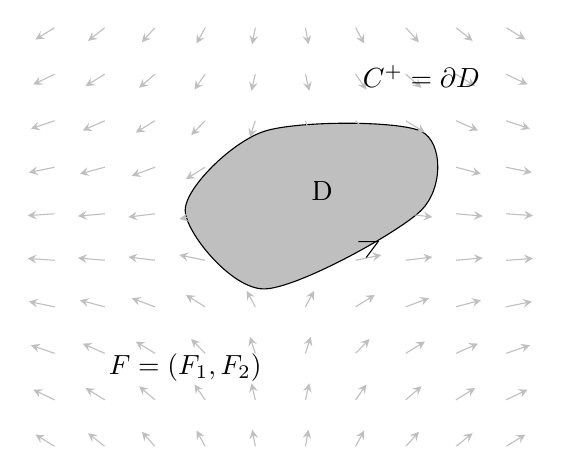
\begin{tikzpicture}
			\draw[fill=lightgray] plot [smooth cycle] coordinates {(2,3) (3,4) (5,4) (5,3) (3,2)};
			\node [above left] at (4,3) {D};
			\begin{axis}[view={0}{90}, hide axis, zmin=-1, zmax=1, tick label style={font=\tiny}]
			\addplot3 [lightgray,-stealth,samples=10,
					quiver={
							u={3*x/pow(x^2 + y^2,1/2)},
							v={-2*y/pow(x^2 + y^2,1/2)},
							scale arrows=0.2,
					},] {0};
			\end{axis}
			\node at (2,1) {$F = (F_1, F_2)$};
			\node at (5,4.7) {$C^+ = \partial D$};
			\draw (4.3,2.4)--(4.45,2.6)--(4.2,2.6);
		\end{tikzpicture}
		\end{center}
  \end{theorem}
		
  Green's theorem has many applications in physics. For example, in order to solve two-dimensional flow integrals measuring the sum of fluid outflowing from a volume, Green's theorem allows us to calculate the total outflow summed about an enclosing area . 
		
  \begin{corollary}
		Let $D$ be a region for which Green's theorem applies with positively oriented boundary $\partial D$. Then, the area of $D$ can be computed with the formula
		\begin{equation}
			A(D) = \frac{1}{2} \oint_{\partial D} x \, d y - y \, d x
		\end{equation}
  \end{corollary}
		
  Green's theorem can be used to determine the area of centroid of plane figures solely by integrating over the perimeter. 
		
\subsection{Stokes' Theorem}
		
  Green's theorem relates line integrals to double integrals. Stokes' theorem generalizes Green's theorem by relating line integrals to surface integrals of 2-dimensional surfaces embedded in $\mathbb{R}^3$. 
		
  \begin{theorem}[Stokes' Theorem]
		Let $S$ be an oriented regular surface defined by paramaterization $\varphi: D \subset \mathbb{R}^2 \to \mathbb{R}^3$, and let the image of the boundary $\partial D$ under $\varphi$ be the boundary $\partial S$ of $S$. 
		
		\begin{figure}[H]
			\centering
			\begin{tikzpicture}
				\begin{axis}[
					view={125}{22},
					axis lines=center,
					xmin=-0.2, xmax=5.6,
					ymin=-0.2, ymax=6.6,
					zmin=0, zmax=2.4,
					ticks=none,
					width=9cm,
					height=7cm,
					colormap/viridis,
					clip=false,
					disabledatascaling % Disables the massive internal scaling causing the crash
				]
					\addplot3[
						surf,
						domain=0:360,
						y domain=0:1,
						variable=u,        % Removed backslash
						variable y=r,      % Removed backslash
						samples=18,
						samples y=5,
						point meta=z,
						mesh,
						draw=black!45,
						shader=flat
					]
					({4 + 1.9*r*cos(u)}, {6.6 + 2.35*r*sin(u)}, {2.55 - 0.45*r^2});
		
					\addplot3[
						blue!70!black,
						line width=0.9pt,
						domain=35:395,
						variable=u,        % Removed backslash
						samples=40,
						postaction={decorate},
						decoration={
							markings,
							mark=between positions 0.125 and 0.875 step 0.05 with {\arrow[scale=1.5]{stealth}}
						}
					]
					({4 + 1.9*cos(u)}, {6.6 + 2.35*sin(u)}, {2.10});
		
					\addplot3[thick, -stealth]
					coordinates {(4,6.6,2.55) (4,6.6,3.25)};
		
					\node at (axis cs:4.95,7.45,2.58) {$S$};
					\node[blue!70!black] at (axis cs:5.15,5.05,2.08) {$\partial S$};
					\node[right] at (axis cs:4,6.6,3.28) {$n$};
				\end{axis}
			\end{tikzpicture}
			\caption{The orientation unit vector $n$ of $S$ induces the positive orientation of $\partial S$, denoted $\partial S^+$. Visually, if you are walking along the curve with your head is pointing in the same direction as the unit normal vectors while the surface is on the left then you are walking in the positive direction on $\partial S$. }
		\end{figure}
		
		Given that $F$ is a $C^1$ vector field defined on $S$, then
		\begin{equation}
			\iint_S \curl{F} \cdot dS = \iint_S \big( \nabla \times F \big) \cdot d S = \oint_{\partial S^+} F \cdot d s
		\end{equation}
		If $S$ has no boundary, that is, if the image of $p^\prime = \partial S$ is not a simple closed curve, then the integral is $0$. 
  \end{theorem}
		
  The above theorem implies that the vector surface integral of a surface without a boundary (i.e. a closed graph, such as a sphere) is always $0$ along the curl of any $C^1$ field. Geometrically, this means that given a closed solid $S$ with field $\nabla \times F$, the rate of flow of the vector field into $S$ is equal to the flow out of $S$. 
		
\subsection{Gauss' Theorem}
		
  The divergence theorem relates the flux of a vector field through a closed surface to the divergence of the field in the volume enclosed. 
		
  \begin{theorem}[Gauss' Divergence Theorem]
		Let $V$ be a subset of $\mathbb{R}^3$. Denote by $\partial V$ the oriented closed surface that bounds $V$ (with outward pointing normal orientation vectors), and let $F$ be a $C^1$ vector field defined on a neighborhood of $V$. Then, 
		\begin{equation}
			\iiint_V \Div{F} \, d V = \iiint_V (\nabla \cdot F) \, d V = \oiint_{\partial V} F \cdot d S = \oiint_{\partial V} (F \cdot n) \, dS
		\end{equation}
		where the two left-most integrals are volume integrals, and the two right-most integrals are surface integrals. 
		
		\begin{figure}[H]
			\centering 
			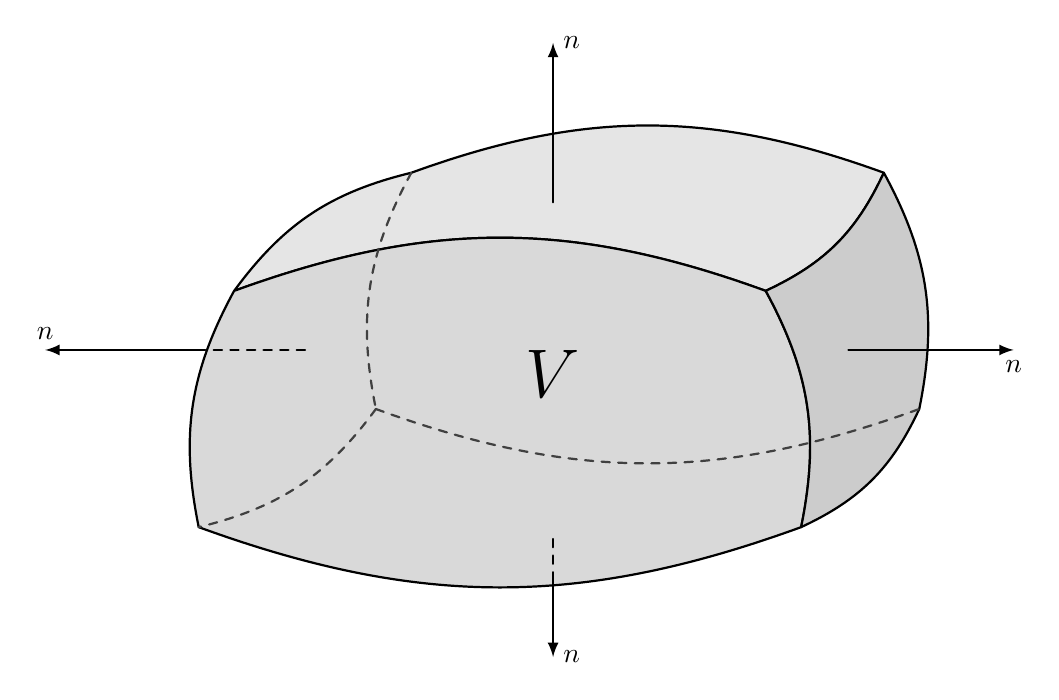
\begin{tikzpicture}[
					scale=1.5,
					line join=round,
					line cap=round
				]
					% 1. Coordinates for the 8 corners of the blob
					\coordinate (FL) at (-2.5, 0.5);   % Front Top Left
					\coordinate (FR) at (2.0, 0.5);    % Front Top Right
					\coordinate (FBL) at (-2.8, -1.5); % Front Bottom Left
					\coordinate (FBR) at (2.3, -1.5);  % Front Bottom Right
			
					\coordinate (TL) at (-1.0, 1.5);   % Back Top Left
					\coordinate (TR) at (3.0, 1.5);    % Back Top Right
					\coordinate (BBL) at (-1.3, -0.5); % Back Bottom Left
					\coordinate (BBR) at (3.3, -0.5);  % Back Bottom Right
		
					% 2. Fill visible faces with flat shades of gray
					% Top face
					\filldraw[fill=gray!20, draw=black, thick] 
						(TL) to[bend left=20] (TR) 
						to[bend left=20] (FR) 
						to[bend right=20] (FL) 
						to[bend left=20] cycle;
				
					% Front face
					\filldraw[fill=gray!30, draw=black, thick] 
						(FL) to[bend left=20] (FR) 
						to[bend left=20] (FBR) 
						to[bend left=20] (FBL) 
						to[bend left=20] cycle;
				
					% Right face
					\filldraw[fill=gray!40, draw=black, thick] 
						(FR) to[bend right=20] (TR) 
						to[bend left=20] (BBR) 
						to[bend left=20] (FBR) 
						to[bend right=20] cycle;
		
					% 3. Draw dashed hidden lines (back and bottom edges)
					\draw[dashed, darkgray, thick] (TL) to[bend right=20] (BBL);
					\draw[dashed, darkgray, thick] (BBL) to[bend left=20] (FBL);
					\draw[dashed, darkgray, thick] (BBL) to[bend right=20] (BBR);
		
					% 4. Draw Normal Vectors (Orthogonal to the viewing plane)
					\tikzset{normal vector/.style={-latex, thick, black}}
			
					% Top normal
					\draw[normal vector] (0.2, 1.25) -- (0.2, 2.6) node[right] {$\boldsymbol{n}$};
			
					% Bottom normal (partially hidden inside the volume)
					\draw[dashed, thick] (0.2, -1.6) -- (0.2, -1.9);
					\draw[normal vector] (0.2, -1.9) -- (0.2, -2.6) node[right] {$\boldsymbol{n}$};
			
					% Left normal (partially hidden inside the volume)
					\draw[dashed, thick] (-1.9, 0) -- (-2.8, 0);
					\draw[normal vector] (-2.8, 0) -- (-4.1, 0) node[above] {$\boldsymbol{n}$};
			
					% Right normal (starts on the right face surface)
					\draw[normal vector] (2.7, 0) -- (4.1, 0) node[below] {$\boldsymbol{n}$};
		
					% 5. Center Volume Label 'V'
					\node at (0.2, -0.2) {\Huge $V$};
			\end{tikzpicture}
			\caption{} 
			\label{fig:gauss_theorem}
		\end{figure}
  \end{theorem}
		
	Intuitively, this makes sense; the volume integrals represent the total of the sources in volume $V$, and the right hand side represents the total flow across the boundary $\partial V$. 
